In this chapter, we describe several prototype applications that we have developed using the behavioral watchpoint framework. These applications provide debugging facilities for kernel modules and demonstrate the effectiveness of the behavioral watchpoint framework. This chapter uses the term \emph{object} to refer to a range of memory locations that are allocated together as a unit.



%To demonstrate the effectiveness of behavioral watchpoint framework, we developed the prototype applications providing debugging facilities for the kernel modules. In these chapter, I used the term \emph{object} to refer to a range of memory locations that are allocated together as a unit.

%to describe a value or aggregate of values stored in memory and referenced by a memory address.

\section{Buffer Overflows \label{sec:buffer_overflows}}
A buffer overflow occurs when a program---in an attempt to write to some object's memory---actually writes to adjacent memory cells. A low-level programming language like C provides raw memory pointers, permits pointer arithmetic, and does not check bounds when accessing arrays. This can result in very efficient code, but the unfortunate side-effect is that accidentally accessing wrong memory is a very common programming error.

The most obvious example in this class of errors is exceeding the bounds of an array. However the bounds of non-array data objects such as heap blocks, C structs, and stack frames, can also be violated. We consider any memory access that falls outside its intended memory range as bound errors. These errors are not difficult to introduce, and they can cause several bugs, some of which can be extremely subtle and lurk undetected for years. Because of this, tools for preventing and identifying them are extremely useful. 

Existing solutions such as Memcheck~\cite{Memcheck} and \emph{fat pointers}~\cite{BccFatPointers}, provide a powerful facility for detecting bounds errors. \emph{fat pointers} hold meta-data for each pointer with the pointer. This metadata describes the memory ranges the pointer can legitimately access and any access via a pointer that is outside its legitimate range is flagged as an error. Another method of detecting buffer overflows relies on the compiler to allocate ``poisoned" regions of memory around each object \cite{AddressSanitizer}. Small overflows (e.g., off-by-one errors) are detected by this approach because they access poisoned memory. Large overflows that ``skip" over poisoned memory and access nearby memory objects are not detected.

Our implementation of a buffer-overflow detector takes an approach similar to \emph{fat pointers} but we store the meta-information for each object in its watchpoint descriptor. Our insight is that unrelated objects will have different base addresses (i.e., the address of one object will not be derived from the base address of another), and thus each object can be distinguished and uniquely identified with a separate watchpoint address, even when objects are adjacent to each other.

%to an unwatched one, or one with a distinct watchpoint, without conflict.
%\emph{addresses} stored in hardware registers, like high-level programming language variable names, are typically not used to simultaneously access two unrelated objects.
%Accessing poisoned memory is an error because it does not exist as a named program entity. However, 
%Our approach is similar in that memory adjacent to a watched object is considered poisoned; however, we do not rely on compiler support, nor do we allocate or mark poisoned memory as such.

\begin{figure}
\begin{lstlisting}[language=C,basicstyle=\footnotesize\ttfamily]
FUNC_WRAPPER(__kmalloc, (size, flags), {
  void *addr = __kmalloc(size, flags);
  ADD_WATCHPOINT(addr, size);
  return addr;
})
\end{lstlisting}
\vspace{-10pt}
\caption[Function wrapper for kernel memory allocator.]{\label{fig:kmalloc_wrapper}Definition of the \texttt{\_\_kmalloc} function wrapper in Granary. The above code expands into a function for wrapping the \texttt{\_\_kmalloc} allocator. Calls to \texttt{\_\_kmalloc} are transparently substituted with calls to the generated wrapper. The wrapper invokes the original \texttt{\_\_kmalloc} function and returns a watched version of the allocated address.}
\end{figure}

We employ three overflow detection policies: heap-based, type-based and stack-based. All three policies depend on the same extension to the meta-information associated with watchpoint descriptors: a \emph{limit address}. Together, the base address (stored in the descriptor) and the limit address delineate an object's boundaries in memory \cite{BccFatPointers}.


\subsection{Heap-based overflow detection\label{sec:heap_overflow}}
The heap-based detection policy detects buffer overflow errors on all heap-allocated objects. We use Granary to wrap the kernel's memory allocators (e.g., \texttt{kmalloc}) and add watchpoints to the addresses returned by those allocators, as shown in \Figref{kmalloc_wrapper}. The lifetime of an added watchpoint is tied to the lifetime of the memory it watches. Each watchpoint's descriptor records bounds information about the allocated memory in the form of the object's base and limit address \cite{BccFatPointers}. A buffer overflow is detected when a dereference of a watched address occurs outside of the bounds recorded by the watchpoint's descriptor (\Figref{detect_overflow}). 
The memory operand-size-specific vtable functions help catch corner cases where memory reads or writes access both an object and its adjacent memory cells, as shown in case $(3)$ of \Figref{detect_overflow}.

%intersect an object's memory and the adjacent memory cells.
%The vtable functions used by these watchpoints detects buffer overflows when a dereference of a watched address 
%memory dereferenced in a read or write falls outside of the bounds
We use Granary to substitute invocations of the kernel's memory allocators (e.g. \texttt{kmalloc}) with wrapped versions of the allocators (\Figref{kmalloc_wrapper}). A wrapped allocator invokes the original allocator but returns a watched version of the allocated address. The lifetime of the watchpoint is associated with the lifetime of the objects and watchpoint descriptor gets collected when objects get freed. 
The watched address returned has its descriptor initialised with the base address as the allocated address and with the limit address as the base address plus the requested allocation size. All buffer overflow detecting watchpoints are initialised with the same vtable pointer, which points to a table of memory operand size-specific functions. The operand size is necessary to detect dereferences of memory that overlap both the object and its adjacent memory, as illustrated in case \emph{(3)} of \Figref{detect_overflow}. The vtable function corresponding to the memory operand size is invoked when a watched address is dereferenced. Each vtable function is programmed to check the watched address against the base and limit addresses stored in watchpoint's descriptor (\Figref{detect_overflow}). If a buffer underflow or overflow is detected then the vtable function notifies the run-time system.

\begin{figure}
\abovedisplayskip=0pt
\belowdisplayskip=0pt
\begin{center}
	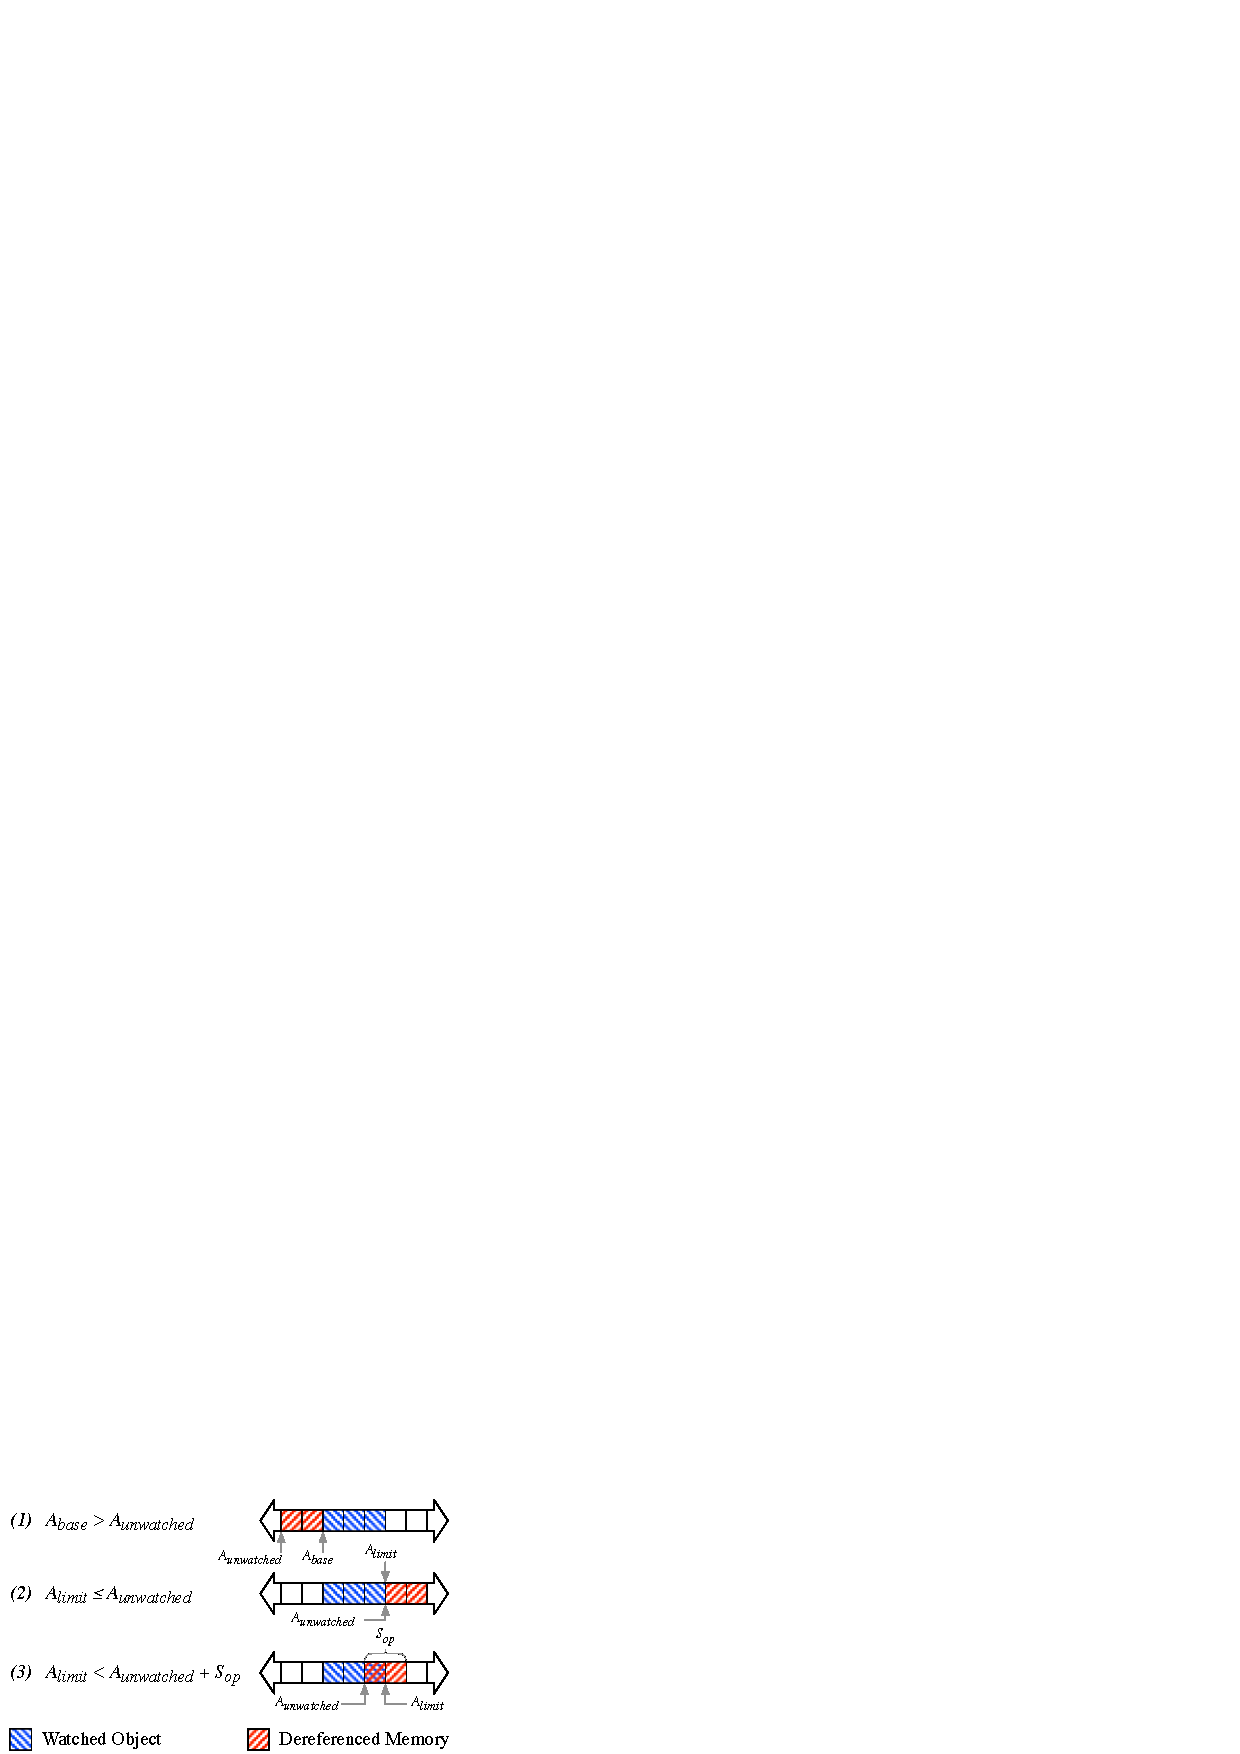
\includegraphics[width=4.5in]{overflow.pdf}
\end{center}
\iffalse
	\abovedisplayskip=0pt
	\belowdisplayskip=0pt
	\begin{align*}
		A_{base}  & > {A_{unwatched}} \tag{Underflow} \\
		A_{limit} & \leq {A_{unwatched}} \tag{Overflow} \\
		A_{limit} & < {A_{unwatched}} + S_{op} \tag{Overlap}
	\end{align*}
\fi
\caption[Buffer overflow detection]{\label{fig:detect_overflow}Three common buffer overflow cases are illustrated above: 1) underflow 2) overflow, and 3) overlap. Beside each illustration is the policy that detects the specific bug. When a watched address ($A_{watched}$) is dereferenced, a vtable function that is specific to the memory operand size ($S_{op}$) is invoked. This function detects a buffer overflow if the intended referenced memory address ($A_{unwatched}$) does not fall within the boundaries delineated by the base and the limit addresses ($A_{base}$ and $A_{limit}$, respectively).}
\end{figure}

\subsection{Type-based overflow detection\label{sec:type_overflow}}
Type-based overflow detection is applied when the type of an object is known. It is distinguished from heap-based overflow detection in that it can apply both to heap and non-heap memory, and it can be used to inform the run-time system about more accurate bounds information. In all other respects, the type-based overflow detection policy detects bugs in the same way as the heap-based policy (as might be encoded within the fields of a vector-like data structure). If the type of an object is known then it can reveal semantic relationships which can enable further type- or heap-based overflow detection. For example, the fields within a structure might encode memory bounds information (as would be the case for a vector-like data structure)

%The type-based detection policy is applied when the type of a pointer is known (i.e., not \texttt{void*}). 
The simplest use case of type information is to infer the limit address of a typed pointer. A more complex use case arises when the fields within a structure encode memory bounds information. In both cases, the vtable functions for typed and untyped memory operate in the same way.
The type of an addressable object becomes known to Granary in the context of a wrapped function. The run-time system performs a type-specific initialisation of a watchpoint's descriptor when a watchpoint is added to a pointer/address with a known type. Type-specific descriptor initialisation is a powerful feature because it allows for new watchpoints to be lazily added (thus propagating our detection capabilities) to newly discovered objects referenced \emph{within} an object of a known type. We automatically propagate type-based watchpoints using type specifications generated from parsing \texttt{C} header files. %Some manual post-processing is required if one is to inform the system of semantic relationships between function arguments or structure fields.

%use a type-specific vtable instead of a generic vtable when watching a typed pointer. Granary includes a database of 


Granary recursively follows argument and return value pointers based on object type specifications. These specifications tell Granary how to follow pointers and what--if any--pointers should be converted to watchpoints. To reduce programmer effort, Granary automatically generates type specifications and wrapper functions for any set of known types and functions. Some manual post-processing is required if the analysis/debugging application needs to understand semantic relationships between function arguments or structure fields. %\comment{Automating this process was an important goal of Granary because of Granary wraps all (approx. 6,000) exported kernel functions.}.



\subsection{Stack-based overflow detection}
Detecting stack overflows is important because they are commonly used in remote code execution and privilege-escalation attacks against operating systems \cite{SecureProgramExecFlowTracking}.
We detect overflows on stack allocated objects when memory outside of the bounds of the activation/call frame in which the object is allocated is accessed. This policy is distinguished from the heap- and type-based policies in that the watchpoint descriptor is managed separately from the watched memory, and the lifetime of the descriptor extends beyond the lifetime of the watched memory.

To detect stack overflows, we view the memory occupied by the activation frame of an invoked function as a dynamically-sized buffer. Like our other buffer overflow policies, we use a watchpoint to detect accesses to memory outside of this buffer. Unlike our other policies, we only \emph{associate} a descriptor with this buffer, and rely on a different mechanism to \emph{add} the watchpoint to stack addresses.
%, and manage what addresses are watched with this descriptor using a separate mechanism.
We separate adding watchpoints from allocating descriptors for stack overflow detection. In particular, we associate a descriptor with the buffer represented by the activation frame of a called function. This descriptor tracks the bounds of the frame over the lifetime of the function call.

We update the bounds of the frame (in the descriptor) when the frame grows or shrinks. When a function returns, the descriptor's bounds shrink to zero, but the descriptor remains allocated. We detect the two most common sources of stack overflows. First, if we see an instruction that copies the stack or frame pointers, then we assume that the copied address can escape the function. A stack address escaping a function is a potential stack-overflow risk. Adding the frame's watchpoint to this address \emph{taints} the copied address. Future copies or displacements of the watched address implicitly propagate its taintedness because offsets of a watched address reference the same descriptor. A dereference of an escaped pointer---even one happening after the function has returned---is detected as an overflow because the watchpoint descriptor remains live. Second, if we see an indexed dereference of the stack or frame pointers that uses a dynamically bound index, then we assume that the effective memory address accessed is a potential stack-overflow risk. We instrument the dereferencing instruction to add the frame's watchpoint to the effective address before the address is dereferenced.


%more support from Granary's run-time system. At a high level, each activation frame is assigned a dedicated watchpoint when a function is called. The effect of an instruction that grows or shrinks an activation frame's size is reflected by a similar change to the base address\footnote{The run-time call stack on x86 grows into lower memory.\comment{ Modifying the base address instead of the limit address allows us to maintain one set of vtable functions for all three buffer overflow detection policies.}} of the frame's watchpoint descriptor. When a function returns, the descriptor of its activation frame is cleared, but remains allocated\footnote{Reclaiming/reusing allocated but unlikey-to-be-used watchpoints is challenging. One overflow-specific approach is to ensure that the next use of the watchpoint is for a buffer whose bounds do not intersect with the current use's bounds. Another approach is to use some number of context switches as a grace period in which the watchpoint cannot be reused, but after which it can be reused. We leave this as future work.} lest the address of a local variable escape the function\footnote{If the address of a stack-allocated object escapes its function activation frame, then that pointer is said to be \emph{dangling}. Dereferences of dangling pointers can cause stack overflow errors. In the kernel, data stored in unallocated stack memory (e.g., through a dangling pointer) is at risk of being clobbered by interrupt stack frames and by function activation frames.}.  

%We assume that a memory instruction operating on a constant displacement of the stack or frame pointer registers is well-behaved. However, if the stack or frame pointer registers participate in a memory instruction and the displacement from the register is dynamically-bound then that instruction is suspect. An instruction that copies the address in the stack or frame pointer registers is also suspect because the copied address might escape the current function or participate in a local stack overflow. All suspect instructions are translated to transparently add the frame's dedicated watchpoint to the dereferenced or copied address.

%This scheme segments the runtime stack into contiguous but non-overlapping regions of watched memory. A straightforward extension excludes saved return addresses and link pointers from the known bounds of activation frames, thus detecting return-oriented buffer overflow attacks.

\begin{figure}[t]
\begin{center}
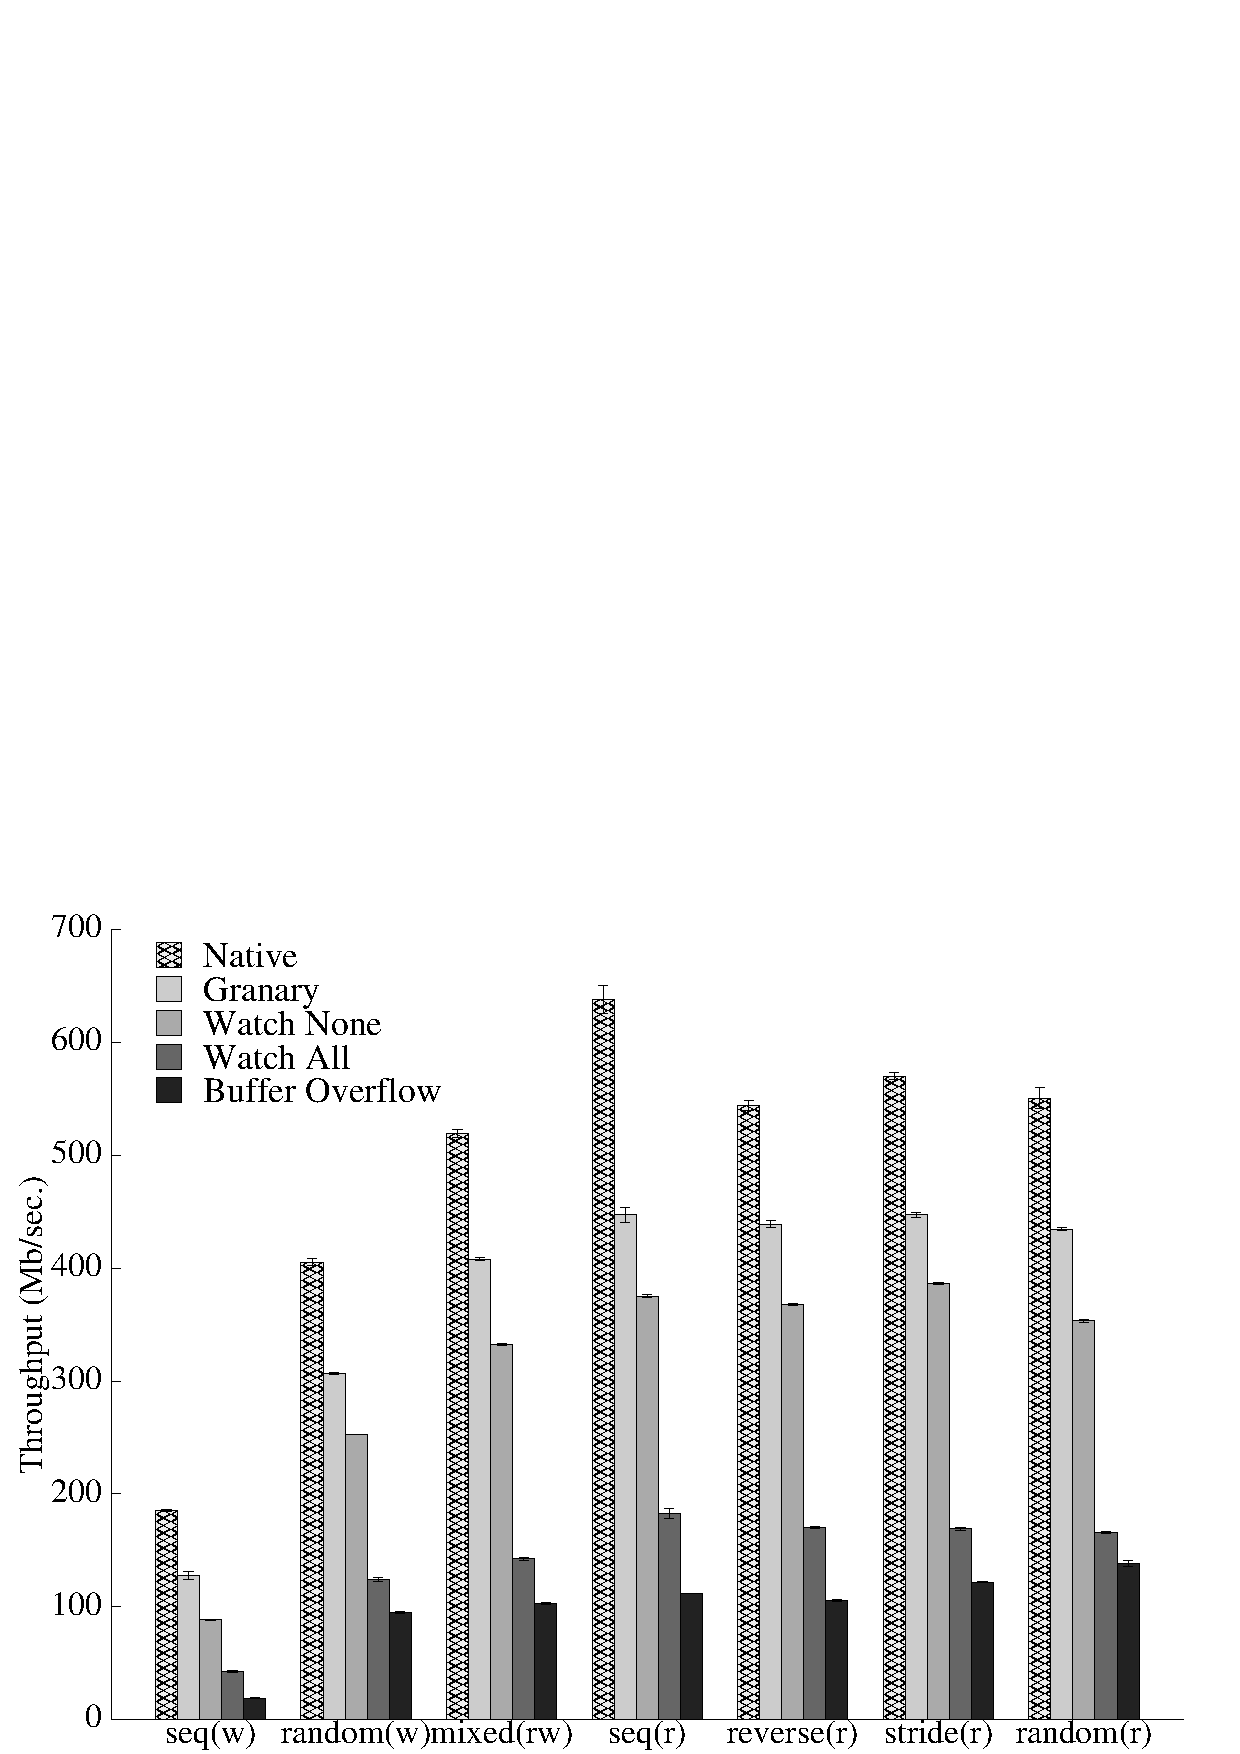
\includegraphics[width=5.0in]{watchpoint_overflow.pdf}
\end{center}
%\vspace{-15pt}
\caption[Performance impact of buffer overflow detector.]{\label{fig:watchpoint_overflow}Performance overhead (Throughput in MB/sec of common file system operations) of buffer overflow detector when used to detect the buffer overflow in \texttt{ext3} file system module. The buffer overflow detector uses code centric instrumentation for the module code and data centric instrumentation for the kernel code. The overflow detector watches all the memory allocated by the \texttt{ext3} and \texttt{jdb} modules.}
%for the watched address is shown.}
\end{figure}


\begin{table*}
\begin{center}
\begin{tabular}{|l|c c c c|}
  \hline
  Benchmark & Native & Watchpoint Null & Everything watched & Buffer overflow\\
  \hline
  Microbenchmark  & 1x & 2.7x & 3.8x & 20x\\
  \hline
\end{tabular}
\caption[Performance impact of buffer overflow detector on microbenchmark]{\label{table:overflow-benchmark}The overhead of watchpoint instrumentation for buffer overflow detector on microbenchmark shown in \Figref{microbenchmark}. The buffer overflow detector uses instrumentation for bounds checking on the access of watched objects.}
\end{center}
\end{table*}


\subsection{Evaluation}
We evaluated the performance of our buffer-overflow detector using a the synthetic microbenchmark shown in \Figref{microbenchmark} and measured the performance of common filesystem operations on an in-memory disk using the \emph{iozone} filesystem benchmark. We used the same experimental setup as described in Section~\ref{sec:approach_eval}. The overhead of the buffer-overflow detector on synthetic microbenchmark is shown in Table~\ref{table:overflow-benchmark}. The high overhead of detector is due to the instrumentation needed for precise bounds checking. \Figref{watchpoint_overflow} shows the overhead of the buffer-overflow detector on the throughput of common filesystem operations issued by the \emph{iozone} file system benchmark. We saw {\texttildelow}80\% drop in the throughput of file system operations. Much of these overhead comes because of code centric instrumentation and the overflow detector watches all the module allocated objects. Watching selected objects for buffer overflow detection will improve its performance.



%\subsection{Real World Results}
%overhead was \texttildelow 21{\footnotesize$\times$}, which is caused by the instrumentation needed for precise bounds checking.


%and measured the performance of common filesystem operations on an in-memory disk.

\section{Selective Memory Shadowing\label{sec:uninitialised_memory}}

Shadow memory enables a program analysis tool to track the history of every memory location and/or value in memory. Existing tools that use shadow memory such as Memcheck~\cite{Memcheck}, TaintCheck~\cite{NewsomeS05}, TaintTrace~\cite{Cheng:2006:TEF:1157733.1157903}, and Eraser~\cite{Savage:1997:EDD:265924.265927} demonstrate that shadow memory is a powerful and widely used method for developing program debugging applications. 


Memcheck~\cite{Memcheck} uses shadow memory to track what allocation/deallocation operations have affected each memory location, and can thus detect accesses to unaddressable memory. It also tracks the undefined memory locations (uninitialised or derived from undefined locations) and can therefore detect dangerous uses of undefined memory. TaintCheck~\cite{NewsomeS05} and TaintTrace~\cite{Cheng:2006:TEF:1157733.1157903} are security tools. They track which values are from untrusted (tainted) sources and which values were subsequently derived from them, and can thus detect dangerous uses of tainted values.
%It also remembers which values are undefined (uninitialised or derived from undefined values) and can therefore detect dangerous uses of undefined values. TaintCheck is a security tool. It remembers which values are from untrusted (tainted) sources and which values were subsequently derived from them, and can thus detect dangerous uses of tainted values.
Eraser~\cite{Savage:1997:EDD:265924.265927} uses shadow memory to track which locks are held when a memory location is accessed, and can thus detect when a memory location is accessed without a consistent lock-set, which may imply a data race. In the above applications, shadow memory provides the ability to detect critical errors, which otherwise could go undetected.

The implementation of shadow memory in these tools is inherently expensive because all memory needs to be shadowed~\cite{Nethercote:2007:SBM:1254810.1254820}. The tools need to maintain extra state for each byte of memory and instrument all loads and stores to keep this state up-to-date. These requirements increase the total amount of code that is run and the program's memory footprint, thus significantly affecting performance. Instead, behavioral watchpoints enable implementing a novel shadowing scheme that allows tracking objects selectively, which decreases the amount of code that needs to be
run and the program's memory footprint.

 %The solution of the problem associated with full memory shadowing is selective shadowing. Selective shadowing allows you to track only the objects of your interested thus decreasing the memory footprints and amount of code required to be run. 



%This makes it important to have an approach which allows you the selective memory shadowing. Selective 
%The previous work on shadow memory is mostly focused on full memory shadowing.



%is implemented in software. However implementing shadow memory correctly is hard because of following three reasons:

%First, the implementation of shadow memory is inherently expensive. A tool need to maintain large amounts of extra state and one shadow byte per byte of live original memory is typical. Most or all loads and stores must be instrumented to keep the shadow memory state up-to-date.% as must operations that affect large regions of memory, such as allocations and deallocations (on the heap or stack ), reads/writes of large areas by system calls, and the loading of the program image into memory at start-up.
%These requirements unavoidably increase the total amount of code that is run, increase a program’s memory footprint, and degrade the locality of its memory accesses. %Shadow memory tools thus typically slow down programs by a factor of 10–100, and shadow memory operations cause much more of this slow-down than other well-studied aspects of tools built with DBI frameworks such as hot trace formation [1] and code cache management [7]


%Second, The robustness of a shadow memory implementation is also important, arguably even more so than its speed. Real world tools must cope with large, uncooperative programs, and if they are to be portable, cannot rely on particular operating system characteristics such as memory layouts. Shadow memory is hard to implement robustly. The shadow memory must be squeezed into the address space alongside the
%original memory in a way that does not conflict with it and does not change the program’s behaviour. This requires considerable flexibility in the shadow memory structure and layout. It also unavoidably reduces the amount of address space a program can use itself,
%which is an important issue on embedded platforms and even 32-bit machines. Obviously, this becomes less of an issue if shadow memory
%can be made smaller, so compact shadow memory is desirable.

%In this section, we show how to use behavioral watchpoints to shadow memory. %Previous work has focused on full memory shadowing \cite{Memcheck}, while
%This section describes about the use of behavioral watchpoints in enabling \emph{selective} shadowing for watched objects. It also describes how the initialisation state of each byte of watched memory is tracked using shadow memory, and how to detect bugs related to the usage of heap-allocated memory. It also discusses the use of selective shadowing in tracking the memory access pattern of the kernel modules.

%Granary provides support to wrap kernel memory allocators and deallocators (e.g., \texttt{kmalloc}, \texttt{kfree}). Wrapped allocators add watchpoints to allocated memory, and wrapped deallocators remove watchpoints before invoking the kernel's deallocators. 
We implement selective shadow memory by maintaining a watchpoint descriptor-specific, variable-sized bitset. %\footnote{As an optimisation, shadow memory for small objects is embedded in the watchpoint descriptor.}. 
Each byte of allocated memory corresponds to one bit of descriptor-specific shadow memory. The bits in shadow memory are initialised to zero. Individual bits are flipped to one by write-specific vtable functions or read-specific vtable functions when a write/read operation happens to the bytes of memory shadowed by those bits. 

%When a wrapped allocator is invoked, a watchpoint is added to the addresses returned by those allocators
 

% in shadow memory are initialised to zero.
%Watchpoints are added to all heap-allocated objects 
%the meta-information within each watchpoint descriptor.
%By tracking the initialisation state, we detect


We use this shadow memory scheme to detect memory error bugs (e.g., uses of uninitialised memory, memory freeing bugs for heap-allocated objects) and to characterize the types of objects accessed by different kernel modules. As described in Section~\ref{sec:heap_overflow}, Granary interposes on the kernel's memory allocators and adds watchpoints to the addresses returned by those allocators. When memory is allocated, the watchpoint descriptor is initialised with the number of allocated bytes (available as an argument to the allocator) and with its own shadow memory. 

%detect uses of uninitialised memory.  Detecting such uses is important because a program using uninitialised memory can exhibit unintended, non-deterministic behaviour.

Uninitialised memory is defined as either allocated memory to which no value has been written, or deallocated memory. We selectively track the initialisation state of each byte of watched memory using \emph{shadow memory} \cite{Memcheck}. Our implementation represents shadow memory as a bitset, where the state of each bit tracks the initialisation state of a byte of watched memory. Watchpoint descriptors are augmented to include the size (in bytes) of a watched object and a pointer to the memory shadowing the object\footnote{As an optimisation, shadow memory for small objects can be embedded in the watchpoint descriptor.}.



\subsection{Read-before-write bugs}
Read-specific vtable functions detect read-before-write bugs by checking if the shadow bit corresponding to one of the read bytes is zero. However, this method of detection can report false positives: it is common for larger-than-needed reads to be performed and for compiler-added structure padding to be read (but never written). A relaxed read-before-write memory checking policy requires that at least one shadow bit is set for every read operation.

\subsection{Memory freeing bugs}
We detect freeing of non-heap memory when the argument to a kernel memory deallocator is not a watched address. We detect an invalid free, such as freeing an offset of an allocated object, when the unwatched address of a watched object being deallocated is different from the watchpoint descriptor's base address. We detect use-after-free bugs by marking the descriptor of a watched address being deallocated as dead. The lifetime of a dead descriptor extends beyond that of the object so that a later use of any watched address with that descriptor will report a use-after-free bug. We detect double-free bugs when the descriptor of a watched address being deallocated is already marked as dead.

%We use Granary to wrap the kernel's deallocation functions (e.g., \texttt{kfree}). Because all allocators are wrapped and add watchpoints, freeing of non-heap memory is easily detected when  

%We detect freeing of non-heap memory 

%If the argument to a wrapped deallocator function is a watched address then the shadow memory for the . 

%Finally, the original deallocator is invoked with the unwatched address as an argument. Reads and writes to a watched address of a deallocated object fail to pass bounds checks because the object size is zero.

Two positive side-effects of our approach is that it detects double-free bugs and freeing of non-heap memory bugs. A double-free is detected when a watched address for an already deallocated object is passed as an argument to a deallocator. An attempt to free non-heap memory is detected when an unwatched address is passed as an argument to a deallocator.

\subsection{Fine-grained access pattern}
Kernel modules execute in the kernel address space with unbounded privileges. These modules are implicitly trusted and interact with each other and the kernel through well defined interfaces and by sharing data in an uncontrolled manner. Unfortunately, the assumed trust leaves commodity OSes vulnerable to malicious and misbehaving kernel extensions\cite{BGI,LXFI, Xu:2004:DEC:1038254.1038305}. We detect the access patterns of the kernel modules using selective shadowing. Behavioral watchpoints tracks the objects of interest and any read/write access to these objects by both the kernel or the module code is captured by the shadow memory. 
The shadow memory information is logged at every control transfer from the kernel to the module. This information is useful for characterizing the access patterns of kernel modules, when may then be used to classify the module to detect module vulnerabilities.
%in a prototype and also detect the vulnerability in the kernel modules.

\section{Memory Leak Detection\label{sec:memory_leaks}}
%Memory leak is a major resource issue which could lead to the malfunctions and negative performance of the system. 
A memory leak occurs when a program does not free dynamically allocated memory or when memory can no longer be referenced. Memory leaks are especially a problem in long running programs, and in operating systems, where memory is lost until the next boot. Existing tools such as Purify~\cite{Rs_purify:fast}, Valgrind~\cite{Seward:2005:UVD:1247360.1247362} and Dr Memory~\cite{Bruening:2011:PMC:2190025.2190067} provide an effective solution for detecting memory leaks in user-space programs but they are not available for the kernel. Other systems such as \emph{kmemleak}~\cite{kmemleak} and SystemTap~\cite{EIgler05architectureof} provide support for debugging memory leaks in the kernel but they operate on the kernel as a whole and not on specific modules of interest.

%one module particularly selected by the user(s).

Implementing a leak detector only for kernel modules is challenging for three reasons. 

First, a leak detector for kernel modules should follow all objects allocated in the module context. Many of these objects should be deallocated by the module. For example, a file system module may make a call to \texttt{create\_workqueue} and allocate a \texttt{work\_struct} that can be used to schedule the delayed work. It is the responsibility of the module to deallocate the object before exit. Keeping track of such objects for a leak detector operating on the entire kernel, such as \emph{kmemleak}, is easy since they track all the memory allocation and deallocation but it is challenging for a leak detector operating only on the kernel module.  

Second, a leak detector needs to perform reachability analysis on all objects allocated in the module context to detect the lost references. Existing leak detectors use different garbage collector algorithm such as reference counting and tracing-based algorithm to detect the live objects. Performing such analysis in only module context is challenging because module regularly lose internal references to the objects that they allocate. For example, a network module can allocate objects and pass with the \texttt{net\_device} structure to the kernel, without retaining references to those objects. The network module can later indirectly access these objects using the kernel's \texttt{netdev\_priv} interface. A whole kernel leak detector, such as \emph{kmemleak}, operating on kernel heaps \& static data can detect such lost references by scanning all allocated objects but a module based leak detector, having limited knowledge of objects allocated in the module context, can not detect the references of such objects and will report them as a leak. 


Third, the existing leak detector in the kernel needs to trace all the memory allocator and deallocator functions in order to track the allocated objects. It also needs to trace the \texttt{container\_of} macros to get the addresses generated from a pre-allocated objects. \emph{kmemleak}, being tightly integrated with the kernel source code, performs this by interposing at the memory allocators/ deallocator (e.g, \texttt{kmalloc}, \texttt{vmalloc}, \texttt{kmem\_cache\_alloc} and other friend functions) and tracing the \texttt{container\_of} operations on pre-allocated objects. Performing such operations by a leak detector, having no knowledge of the kernel activities and operating only on the module binaries is not possible.


%suffers from the false negative because the allocated object doesn't maintain the state information about the memory block. This makes it difficult to identify the transient presence of freed objects in the static or the heap memory. The existing solution of leak detector based on garbage collection algorithm also can not identify the memory leaks due to the increase in stale objects. These stale objects gets allocated by the module but they never gets used and the module also doesn't lose their references. Identifying such objects without tracking the access of each memory block is not possible.


%Tracking the liveness of these objects requires a view on kernel execution which is not normally provided by module-only instrumentation.


 %are challenging because not all module-owned objects are directly allocated by modules. For example, a network driver module may make a call to an skb allocator (to allocate a \texttt{struct sk\_buff}) in an interrupt context when the module code is not running but it is the responsibility of the network module to deallocate them.



%should follow the module-owned objects and reports leak if and when module loses the reference of any of them. An object is defined as module-owned if it is allocated in the module context and it is the responsibility of the module to deallocate the object. However, keeping track of all such objects are challenging because not all module-owned objects are directly allocated by modules. For example, a network driver module may make a call to an skb allocator (to allocate a \texttt{struct sk\_buff}) in an interrupt context when the module code is not running but it is the responsibility of the network module to deallocate them.

%driver module may make a call to an skb allocator (to allocate a struct sk_buff) in an interrupt context when the module code is not running

%We built a memory leak detector for the kernel modules. The leak detector for the kernel modules follow the module owned objects and reports if module loses the references of them. A module owns the objects allocated by them and it is the module's responsibility to deallocate them. However, keeping track of all such objects is challenging because not all module-owned objects are directly allocated by modules. For example, \texttt{sk\_buff} objects used by network modules are allocated by kernel interrupt handlers, but must be deallocated by the network modules. 

%Second, a leak detector performs reachability analysis on all module-owned objects to detect the lost references of the objects. Leak detector uses different garbage collector algorithm such as reference counting and tracing-based algorithm to detect the live object. Performing such analysis in only module context is challenging because module regularly lose internal references to the objects that they own. For example, a network module can allocate objects and pass with the \texttt{net\_device} structure to the kernel, without retaining references to those objects. The network module can later indirectly access these objects using the kernel's \texttt{netdev\_priv} interface. Tracking the liveness of these objects requires a view on kernel execution which is not normally provided by module-only instrumentation.

%Third, the existing leak detector suffers from the false negative because the allocated object doesn't maintain the state information about the memory block. This makes it difficult to identify the transient presence of freed objects in the static or the heap memory. The existing solution of leak detector based on garbage collection algorithm also can not identify the memory leaks due to the increase in stale objects. These stale objects gets allocated by the module but they never gets used and the module also doesn't lose their references. Identifying such objects without tracking the access of each memory block is not possible.


 %thus the transient presence of deallocated objects in the  
%In the implementation of leak detector there is a need to track the state of the allocated objects to reduce the false negative. The existing memory allocator/deallocator doesn't maintain a meta-information with each objects. Thus making it difficult to identify the freed objects thus reporting false negative.

We implemented the leak detector for the kernel modules using the watchpoint framework. The challenges involved in implementing a leak detector only for the kernel modules make behavioral watchpoints a suitable solution. Behavioral watchpoints solve the challenges involved in three ways:
\begin{enumerate}[i)]
	\item The watchpoint framework ensures that all objects allocated in the module context are watched. These watched addresses are easily disambiguated from normal memory addresses and integers that look like watched addresses. This is done by taking over all kernel memory allocators and tracking the execution context of the module running under its control. This helps the framework identify the context of every memory allocation and adds watchpoints on all these objects. However, in the process the watchpoint framework may add watchpoints on the objects not related to the module. Adding extra watchpoints on objects does not affect the correctness of the leak detector. We detect such objects during the collector scan and suppress the false positive that may get reported due to them.

	\item Behavioral watchpoint solves the problem of losing internal reference of objects allocated in the module context by providing leak detector complete visibility of the watched objects. Any read/write accesses performed on these watched objects get detected by the watchpoint instrumentation or the hardware traps which attaches the instrumentation framework with running code. The read/ write operations on watched addresses mark these objects live and the collector scan considers these objects as reachable. The ability to track the accessed objects is particularly helpful in detecting stale objects that are potentially leaked. The leak detector based on garbage collector algorithm such as \emph{kmemleak} can not detect such objects.

	\item Behavioral watchpoints help associate the allocated object with the descriptors. The descriptors hold meta-information for each objects and help identifying the state of a memory block without much of the effort. This helps leak detector limit the scope of scanning to objects that are allocated and live. The behavioral watchpoints are also viral and every addresses derived from a watched addresses (e.g., through copying or offsetting) is also watched. The watchpoint framework does not need to trace the pointer arithmetic used to derive addresses from the allocated objects. \emph{kmemleak} reports false positive if the program uses other than \texttt{container\_of} operations to generate derived addresses. %to track the derived addresses from the% It also helps in tracking the read/write access of the watched objects by kernel or the module code.
\end{enumerate}


%Behavioral watchpoints are viral and every addresses derived from a watched addresses (e.g., through copying or offsetting) is also watched.

%Our approach ensures that all module-owned objects are watched when allocated. Leak detector ensures this by taking over all the kernel allocators and tracking every entry and exit from the kernel to the module and vice-versa. This helps us in identifying if the allocation is happening in the module context or not. We add watchpoint with all the objects allocated in the module context. 
%\texttt{call} from kernel to the module code and \texttt{ret} from the module to the kernel.   
%We ensure this by hot-patching all the kernel allocators and tracking all the calls from the module to the kernel which reaches to the allocators and add watchpoint with those objects. 
%Behavioral watchpoints solve this problem of losing the internal reference of the module-owned object by giving the leak detector visibility into kernel accesses to watched objects, which trigger hardware traps that attach instrumentation to the kernel code. This instrumentation marks kernel-accessed watched objects as live. The implementation of leak detector benefits from using watchpoints in three ways: 
%\begin{enumerate}[i)]
	%\item watched addresses are easily disambiguated from normal memory addresses and integers that look like watched addresses;
%        \item the scope of scanning can be limited using the meta-information provided by descriptors
	%\item descriptors provide meta-information that allows our system to limit the scope of scanning; and
	%\item scanning can stop if all watched objects are reached.
%\end{enumerate}




%A conventional approach of implementing leak detector is to perform the reachability analysis on the module-owned objects. The existing solution, \emph{kmemleak} uses mark/sweep algorithm \cite{Boehm:1991:MPG:113445.113459} on kernel memory to detect if/when module-owned objects become unreachable starting from a set of ``root'' objects. This is challenging because modules regularly lose internal references to the objects that they own. For example, a network module can allocate objects and pass with the \texttt{net\_device} structure to the kernel, without retaining references to those objects. The network module can later indirectly access these objects using the kernel's \texttt{netdev\_priv} interface. Tracking the liveness of these objects requires a view on kernel execution not normally provided by module-only instrumentation.

%We used behavioral watchpoints to implement memory leak detector. Our approach ensures that all module-owned objects are watched when allocated. Behavioral watchpoints solve this problem of losing the internal reference of the module-owned object by giving the leak detector visibility into kernel accesses to watched objects, which trigger hardware traps that attach instrumentation to the kernel code. This instrumentation marks kernel-accessed watched objects as live. The implementation of leak detector benefits from using watchpoints in three ways: 
%\begin{enumerate}[i)]
%	\item watched addresses are easily disambiguated from normal memory addresses and integers that look like watched addresses;
%        \item the scope of scanning can be limited using the meta-information provided by descriptors
%	\item descriptors provide meta-information that allows our system to limit the scope of scanning; and
%	\item scanning can stop if all watched objects are reached.
%\end{enumerate}

%More operationally, a dynamically-live heap object is one
%that can be reached by following pointers that will be dereferenced in the future of
%the computation (dynamically-live pointers). In order to retain only dynamically-live
%objects, the ideal garbage collector must be able to exactly identify what memory locations contain dynamically-live pointers.

\subsection{Object Liveness Analysis}\label{sec:object_liveness}
The effectiveness of a leak detector in identifying the object leaks depend on the ``accuracy'' of the liveness analysis. An ideal leak detector identifies all heap-allocated objects that are not dynamically live and reports them as leak. A dynamically-live heap object is one that can be reached by following pointers that may be dereferenced in the future. 

Existing leak detector solutions such as \emph{kmemleak}~\cite{kmemleak}, Purify \cite{Rs_purify:fast} and Dr Memory \cite{Bruening:2011:PMC:2190025.2190067} use a garbage collection algorithm to perform object liveness analysis. They use the mark/sweep collector algorithm \cite{Boehm:1991:MPG:113445.113459} to detect reachability of the allocated objects starting from a set of ``root-set'' objects. Their root-set includes system registers and non-heap addressable memory. 

They perform reachability analysis periodically at intermediate position and it involves stopping the client when collector\footnote{A low priority daemon thread which runs intermittently in the background performing reachability analysis on the allocated objects} is in process. However, the solution is not very efficient when client operates on a large number of heap-allocated objects, such as is typical in operating systems. It stops the client for longer time. 

One solution for reducing the pause time is to use generational or parallel collection. Generational collection avoids stop-the-world by running the collector thread occasionally but it doesn't remove the problem completely. However the parallel collectors take an orthogonal approach and reduce the time of pause by running the collector in parallel to the client.


In our implementation of leak detector we used the parallel collector to perform object liveness analysis. Keeping in view of the challenges involved in performing object liveness analysis, we used three different policies to perform the leak scan. 

%took middle approach and used mostly-parallel collector~\cite{Boehm:1991:MPG:113445.113459, Barabash:2005:PIM:1108970.1108972} to perform the object liveness analysis. It is called as mostly parallel collector because we update the ``root-set'' in stop the world collector and perform the reachability analysis from these ``root-sets'' by running the collector parallel to mutator (client). 
%The aim of our leak detector is to detect the memory leaks in the kernel modules. These kernel modules execute in a complex and dynamic environment, sharing the data over irregular interface. Many of these shared objects are allocated directly or indirectly by the modules. Behavioral watchpoints provide an efficient solution by providing complete visibility to the module-owned object and making these watched objects easily identifiable, thus limiting the scan space but they does not provide any solution for performing the reachability analysis on all these watched objects. Performing reachability analysis on these objects is challenging because of two reasons. First, these module allocated objects get shared with the kernel over complex and irregular interface making them difficult to track and many of them are reachable only through the kernel internal data structure. The reachability analysis of these objects without accounting the kernel allocated memory is non-trivial and it will lead to false positives. Second, our leak detector framework gets loaded as the kernel modules and it comes into the picture long time after the system ``boot-up''. Without having account of these memory block we can not claim to perform the complete leak scan. Keeping in view of these challenges we used three different policy for performing the leak scan. 


%A conventional approach of implementing leak detector is to perform the liveness analysis on the allocated objects. Existing solution such as \emph{kmemleak}~\cite{kmemleak}, Purify \cite{Rs_purify:fast} and Dr Memory \cite{Bruening:2011:PMC:2190025.2190067} uses garbage collection algorithm to perform object liveness analysis. \emph{Kmemleak} uses mark/sweep algorithm \cite{Boehm:1991:MPG:113445.113459} on kernel memory to detect the reachability of the allocated objects starting from a set of ``root'' objects. The effectiveness of leak detector in identifying the lost objects depends on the accuracy of their object liveness analysis. 
%Existing solution such as Purify \cite{Rs_purify:fast} and Dr Memory \cite{Bruening:2011:PMC:2190025.2190067} leak detector uses garbage collection algorithm to perform liveness analysis. 
%A straightforward implementation of garbage collection algorithm is to implement tracing based collector. It involves stopping the client when collector is in the process performing liveness-analysis. However, this solution is not very efficient when client operates on very large heap-memory as it stops the clients for longer time. The solution to reduce the pause time in tracing algorithm based leak detector is generational or parallel collection. Generational collection avoids stop-the-world time by running the collector thread occasionally, thus doesn't remove the problem completely. However the parallel collectors takes orthogonal approach and reduces the time of pause by running collector parallel to client. We took similar approach of mostly-parallel collector to perform the object liveness analysis.

%In Linux kernel, the module and kernel interacts in a complex ways and there is frequent transfer of shared objects between the kernel and the modules. Many of these shared objects are allocated by the module. Keeping track of the references of these objects with only module view of the objects is non-trivial. This makes it important for the leak detector to track both kernel and the module objects. It was important for us to study the transfer or the ownership of the objects. In our implementation of leak detector we uses three different scan policy to perform the object liveness analysis.

 %following three different liveness analysis policy for the leak detector:

\paragraph{Scanning of accessed objects:} This is an aggressive scanning policy for detecting memory leaks. The approach is similar to bookmarking collectors~\cite{Hertz:2005:GCW:1065010.1065028} and Melt~\cite{Bond:2008:TML:1449764.1449774} which track the accesses of allocated memory blocks to detect stale objects at page or object granularity. The approach considers all objects that are accessed between two consecutive scans as live objects and performs reachability analysis considering them as ``root-sets''. Any object which is not reachable from these objects is considered as stale or a potentially leaked object. 

The leak detector tracks all accesses of the watched objects and updates the meta-information associated with their descriptors. The scanner thread (collector) periodically scans the descriptors stored in a global descriptor table and marks the objects that were accessed in the last epoch as live. The scanner thread later performs reachability analysis considering these objects as ``root-sets''.  The leak detector also tracks the sources of memory allocation in the descriptors and a constant increase in the stale objects from one source is reported a possible leak.


This approach reduces the overhead of leak scan which is performed by the collector periodically and it is also helpful in finding stale objects (dead but reachable) which the existing garbage collector algorithm based leak detector can not detect. However, the approach performs limited reachability analysis, thus resulting in increase in the false positive especially for objects which does not get accessed for longer interval of time. It also can't find the objects with live leak i.e the allocated objects are getting accessed periodically but these accesses are nonetheless useless. Detecting such leaks with any leak detector is challenging.



 %to find the objects which is accessed in last epoch and mark them dead accounting them as live during the scan interval. The approach also tracks the source of each allocation and the constant increase in the stale objects from one source increase the possibility of memory leaks. 

%In this scan policy, every access of the watchpoint objects also updates the meta-information associated with them. The scanner thread periodically scans the descriptor to find the objects which is accessed in last epoch and mark them dead accounting them as live during the scan interval. The approach also tracks the source of each allocation and the constant increase in the stale objects from one source increase the possibility of memory leaks.

%The approach decreases the cost of performing object liveness analysis by the collector and it is also helpful in finding the leaks of stale objects (dead but reachable) which can not be identified using garbage collector algorithm. However, the approach is limited in performing reachability analysis, thus it results in the false positive especially for the objects which doesn't get accessed for long interval of time. The approach also can't find the objects with live leak where the allocated objects gets accessed periodically but these accesses are nonetheless useless. Detecting such leaks in the module is difficult.


%and mark them dead after accounting them as live during the scan interval. The leak detector makes decision after 10 scans.

%The approach deceases the cost of object liveness analysis, but it results in the false positive for those objects which doesn't gets accessed for long period of time.

\paragraph{Scanning of module reachable objects:} 
We define module reachable objects as objects which a module can access directly or has accessed in the past. It includes static data for both the kernel and the modules, system registers, threads stack executing module code and all heap-allocated memory viewed by the module directly or indirectly. Module viewed objects are the objects allocated by the kernel but passed to the module during its course of execution. We keep track of such objects by interposing at the kernel/module interface and collecting all the kernel objects passed to the modules. The type information about these objects helps us in associating a type-specific scanner with each object, which performs deep scanning of these objects during a leak scan.

In this leak scan policy, the collector considers all module reachable objects as the ``root-set'' and recursively scans them to perform liveness analysis. This scan policy uses the mostly-parallel collector~\cite{Boehm:1991:MPG:113445.113459, Barabash:2005:PIM:1108970.1108972} instead of the parallel collector for updating the ``root-set'' before performing the leak scan. This is important to have a consistent snapshot of system registers and thread stack running the module code.  The parallel scanning of kernel objects requires maintaining consistency and avoid the cyclic dependency of dependencies across data structures. We detect cyclic dependencies by hashing each memory block during a scan and storing them in a data structure. The scan of a memory block is stopped if its hash is found. We also use the scan depth as a fall back mechanism to avoid walking a long list of objects in a data structure. In our implementation we used a scan depth of ``6'' which we find is appropriate for detecting all watched objects in any kernel data structure. We are also using relaxed consistency policy during the scan. This is because our leak detector makes a decision about a memory block leak after multiple scans.

This approach reduces false positives compared to the first approach because it includes module-viewed objects in the root set. However, it has a higher cost because it requires maintaining bookkeeping information for the module-viewed objects and tracking their deallocation. The approach does not remove false positives completely as it is not able to track references to objects that are allocated by the module but passed to the kernel, after which the kernel uses internal data structures to maintain references to the objects.

%kernel and kernel uses internal data structure to maintain its references. 

%of object scan by scanning them twice before making a decision. We consider our consistency approach an appropriate because the leak detector makes decision about a memory block after multiple scans.

%where the ``root-sets'' for scan gets updated in stop-the-world collector. This is required to have a consistent snapshot of system registers and thread's stack running the module code. The parallel scan of kernel objects requires to maintain consistency and avoid the cyclic dependency of data structure. We avoid the cyclic dependency by hashing the memory block after every scan and storing them in a data structure. The scan of a memory block gets suspend if its hash is found in the data structure. We also use scan depth as the fall back to avoid walking of the list objects in a data structure. In our implementation we used the scan depth as ``6'' which we find appropriate for detecting the watched objects in the data structure. We relaxed the consistency of object scan by scanning them twice before making a decision. We consider our consistency approach an appropriate because the leak detector makes decision about a memory block after multiple scans.




%The module reachable objects includes the static data for both the kernel and modules, system registers, stack of threads executing module code and all heap-allocated memory viewed directly or indirectly by the module. We defined the module viewed objects as the objects allocated by the kernel but passed to the module during its course of execution. We keep track of all such objects by interposing at the kernel/module interface and each object gets associated with a corresponding type scanner function based on the object types. These type scanner function is used by the collector to recursively scan the object.

%This scanning policy uses mostly-parallel collector where the ``root-sets'' for scan gets updated in stop-the-world collector. This is required to have a consistent snapshot of system registers and thread's stack running the module code. The parallel scan of kernel objects requires to maintain consistency and avoid the cyclic dependency of data structure. We avoid the cyclic dependency by hashing the memory block after every scan and storing them in a data structure. The scan of a memory block gets suspend if its hash is found in the data structure. We also use scan depth as the fall back to avoid walking of the list objects in a data structure. In our implementation we used the scan depth as ``6'' which we find appropriate for detecting the watched objects in the data structure. We relaxed the consistency of object scan by scanning them twice before making a decision. We consider our consistency approach an appropriate because the leak detector makes decision about a memory block after multiple scans.

%The approach decreases the false positive by including the module viewed kernel objects in the ``root-sets''. However, the approach requires to maintain book-keeping of kernel objects passed to the module which has additional cost. The approach also doesn't remove the false positive completely as it is not able to track the references of objects which are allocated by the module but passed to the kernel and kernel uses local data structure to maintain its references. 


%the state data of both the kernel and modules and all the kernel and module heap-allocated object which is viewed directly or indirectly by the module.

%In the initial implementation of leak detector, we decided to track all the in-memory kernel data structure. we track all the module viewed objects. We defined the module viewed objects as the objects passed to the module during its course of execution. We keep track of all such objects and scan them periodically looking for the watchpoints. To maintain the consistency during the data structure we scan them twice and to avoid the circular dependency on the data structure we hash the data structure.

%This policy decreases the false positive but requires to have a lot of book-keeping for the kernel objects. The approach is also not able to track the references of objects which are allocated by the module but passed to the kernel and kernel uses local data structure to maintain the reference of the objects for long time. 

%we studied the ownership transfer of the module owned objects. We track all the object viewed by the module and scan them periodically looking for the watchpoints.





\paragraph{Scanning of kernel heaps and static data:} This is the most conservative policy and used as the fall back approach for performing a leak scan. This policy scans the static data for both kernel and the modules and kernel heaps to find any references to watched objects. A watched object that is not found during the scan is definitely considered a leak.

For scanning kernel pages, we used the kernel page tables and the kernel data structure \texttt{init\_level4\_pgt} to access kernel pages. The scanner thread (collector) divides the kernel pages based on the memory regions and types and scans them based on priority. The scanner thread stops scanning the kernel pages once it finds at-least one reference to watched objects.

This approach avoids any false positives but scanning the kernel heap memory is expensive. Also, the scanning of kernel pages can cause false negatives because leaked objects may have internal pointers containing watched addresses. We reduced the problem by removing the memory block of watched objects that are not live from the scan list.


 %and pointers associated with kernel data structure which is not zeroed out. 


%We reduce the false negative by ignoring the scan of pages associated with watched object and they get scanned only when a reference of that object is found in other pages. This is particularity required as we found in many cases the internal pointers of watched object was initialized with the watchpoint address and scanning of these pages or memory block will provide the false negative even if the object is considered as lost. 

%for implementing leak detector. In this policy we scan the entire kernel heap and module \& kernel static data for finding the references of the watchpoints. Any watchpoints not found during the scan is considered as leak. For scanning the kernel heaps and static data structure we walk over the kernel page table using the page table data structure \texttt{init\_level4\_page}.

%The scanning the kernel heap and static data reduces the chances of false positive but the cost of scanning them is costly. However, In our approach we device the kernel address space in different region and we scan them based on the priority. The scanner thread also stops scanning the memory once it finds at least one reference of all the watched objects.

%The disadvantage of scanning the kernel heaps is that 

%In this can policy we scan the entire heap memory and static data by walking over the page table looking for the watched objects.


%Other solutions such as (...) considers objects staleness as an indicator of problematic behavior.


%The existing leak detector tracks the behavior of the arbitrary objects   

%track behaviors
%of arbitrary objects and report problems when tracked objects
%become suspicious. One major category of work [8, 9, 10, 18, 33]
%considers objects’ staleness (i.e., time elapsed since the program
%last used these objects) as an indicator of problematic behavior,
%while another category [20, 23] treats objects as suspicious if instances
%of their types exhibit sustained growth

%Our approach of leak detector is based on the liveness analysis of heap objects, which are directly or indirectly allocated by the modules. Similar to existing solution like Purify \cite{Rs_purify:fast} and Dr Memory \cite{Bruening:2011:PMC:2190025.2190067}, leak detector uses garbage collection algorithm to detect memory leaks. A straightforward implementation of garbage collection algorithm is to implement tracing based collector. It involves stopping the client when collector is in the process performing liveness-analysis. However, this solution is not very efficient when client operates on very large heap-memory as it stops the clients for longer time. The solution to reduce the pause time in tracing algorithm based leak detector is generational or parallel collection. Generational collection avoids stop-the-world time by running the collector thread occasionally, thus doesn't remove the problem completely. However the parallel collectors takes orthogonal approach and reduces the time of pause by running collector parallel to client. We took similar approach of mostly-parallel collector to perform the object liveness analysis.  

%In our approach of liveness analysis, we use three different analysis policy:



%The leak detector scans kernel memory using the conventional mark/sweep algorithm \cite{Boehm:1991:MPG:113445.113459} to detect if/when module-owned objects become unreachable starting from a set of ``root'' objects. This is challenging because modules regularly lose internal references to the objects that they own. For example, a network module can allocate objects and pass with the \texttt{net\_device} structure to the kernel, without retaining references to those objects. The network module can later indirectly access these objects using the kernel's \texttt{netdev\_priv} interface. Tracking the liveness of these objects requires a view on kernel execution not normally provided by module-only instrumentation. Behavioral watchpoints solve this problem by giving the leak detector visibility into kernel accesses to watched objects, which trigger hardware traps that attach instrumentation to the kernel code. This instrumentation marks kernel-accessed watched objects as live.



%The leak detector benefits from using watchpoints in three ways: %\begin{inparaenum}[i)]
%	\item watched addresses are easily disambiguated from normal memory addresses and integers that look like watched addresses;
%        \item the scope of scanning can be limited using the meta-information provided by descriptors
%	\item descriptors provide meta-information that allows our system to limit the scope of scanning; and
%	\item scanning can stop if all watched objects are reached.
%\end{inparaenum}

%Two key benefits of our watchpoints solution is that watched addresses are easily disambiguated from normal memory addresses, and that we can stop scanning memory if all watched objects are live and reachable.

%Detecting leaks of such objects with a limited view of module is challenging. Behavioral watchpoints provide a way to ensure the visibility of such objects by triggering a hardware trap on its access and mark them as live.
%on memory access of these objects by enabling demand-based translation and marking them as live.


% during device registration. 


%The object becomes invisible to the module and gets accessed through the kernel interface \texttt{netdev\_priv}. This makes it difficult to detect leaks based on module's limited view. Bhavioural watchpoints provides a way to ensure complete visibility on memory access of these objects by enabling demand-based translation and marking them as live.

%All module owned objects are not directly allocated by the module and kernel can allocate it on behalf of the module. 
%All module-owned objects are not directly allocated by the module. For example, a network driver module may make a call to an skb allocator (to allocate a \texttt{sk\_buff} structure) in an interrupt context. Once the buffer is send over the network, it is the responsibility of the network module to deallocate the buffer. In Granary, we use wrappers to add watchpoints at relevant allocators such as \texttt{\_\_alloc\_skb}. The leak detector keeps track of these watched objects and reports possible leaks. 

%Module holds partial view of the kernel and to detect leaked object there is a need to perform reachability analysis on both kernel and module objects. Behavioral watchpoints helps in identifying the objects owned by the module, thus limiting the type of objects which needs to be tracked. Watched object holds descriptor information in high-order bits, making it easy to track the memory state information. This is helpful in identifying live objects and reduces the chance of false positive. The leak detector uses the conventional mark and sweep algorithm and mostly-parallel collector~\cite{Boehm:1991:MPG:113445.113459} to perform the rechability analysis.
 
%Watched addresses are also more easily disambiguated 

%Behavioral watchpoints are important for implementing the leak detector because they help in identifying the objects owned by the module, thus limiting the type of objects that need to be tracked. Each watched object holds the memory state information embedded in its descriptor, making it easy to identify objects that are live and reachable. % from one of the root-sets\footnote{The root-set for leak detector reachability-analysis includes both kernel and module data structures.}. 
%The leak detector uses the conventional mark and sweep algorithm and mostly-parallel collector~\cite{Boehm:1991:MPG:113445.113459} to perform the reachability analysis.


%are easily identifiable because they hold the descriptor table index in high-order bits and 3) Each watched object holds the memory state information with it. Thus making it easy to identify the the objects which are live and reachable from one of the root-sets. The leak detector uses the conventional mark and sweep algorithm and mostly-parallel collector~\cite{Boehm:1991:MPG:113445.113459} to perform the rechability analysis.



%there is a need to perform rechability analysis of all kernel objects, which will have significant cost.



%then gets accessed through the kernel interface and become invisible to the module and is reachable only through the \texttt{net\_device} structure. Bhavioural watchpoints ensures complete visibility of these objects and enables on-demand instrumentation on its access, marking them live.



%Developing a leak detector only for kernel modules is challenging because of following three reasons:
%Our approach is based on performing reachability analysis on module owned objects. 
%Memory leak is a common problem in Linux kernel and its modules \cite{Boehm96simplegarbage-collector-safety}. A serious memory leak in kernel modules can easily make the system unstable this is because every time kernel losses a piece of memory, it can't be reclaimed until next boot. 
%Our approach of detecting memory leaks in kernel module is to perform rechability analysis on the module owned objects. 
%This is challenging because: 

%1) All module owned objects are not directly allocated by the module. For example, a network driver module may make a call to an skb allocator (to allocate a \texttt{sk\_buff} structure) in an interrupt context when the module code is not running. Once the buffer is send over the network, it is the responsibility of the network module to deallocate the buffer.

%2) Module allocates many independent objects which they share with the kernel. Module losses its visibility once such objects are passed to the kernel. For example, a network module during device registration can allocate an object and pass it with \texttt{net\_device} structure. This object then become invisible to the module and is reachable only through the \texttt{net\_device} structure. Detecting leak for such objects requires complete visibility of the kernel. 
%an object and pass it with \texttt{net\_device} structure. 
%till it gets its reference 
% passed to the kernel till it gets his reference back. 
%frequently share with the kernel. Module looses the visibility for such objects till it gets back their references. For example, filesystem module \texttt{ext3} allocates object of type \texttt{inode} and passes it to the kernel. The module holds no reference of the object once it is passed and only 
%loose its visibility for module code till the time kernel passes them back to the module. For example,   
%There is frequent transfer of module allocated objects at kernel/module interface and module may not hold the reference of objects passed to the kernel.  For example, file-system module \texttt{ext3} allocates object of type \texttt{struct inode} and passes it to the kernel. Once it is passed to the kernel module doesn't hold reference of \texttt{struct inode}. Thus having limited view of the module doesn't help in detecting leaks.  

%3) Module only holds partial view of the kernel and much of the module allocated objects are reachable only through the kernel objects. To detect the leaked object there is a need to perform rechability analysis of all kernel objects, which will have significant cost.


%and detect the leaked objects it is needed to perform the rechability analysis on 


%In Granary, we use wrappers to add watchpoints to the relevant allocators (e.g., \texttt{\_\_alloc\_skb, skb\_clone}). The leak detector keeps track of these watched objects and reports possible leak. 

%Behavioral watchpoints are important for implementing the leak detector because: 1) They help in identifying the objects owned by the module, thus limiting the type of objects which needs to be tracked, 2) The watched addresses are easily identifiable because they hold the descriptor table index in high-order bits and 3) Each watched object holds the memory state information with it. Thus making it easy to identify the the objects which are live and reachable from one of the root-sets. The leak detector uses the conventional mark and sweep algorithm and mostly-parallel collector~\cite{Boehm:1991:MPG:113445.113459} to perform the rechability analysis. % from its root-sets. 
%Based on this leak detector divides the watchpoints into three different categories: 
%\begin{enumerate*}
%   \item[i)] Watched objects which are reachable from one of its rootset. They are not considered as leak.  
%   \item[ii)] Watched objects that are not reachable from any of the rootsets are considered as potentially garbage. 

   %Watched objects that are not reachable and never owned by the modules are considered as live. This include objects which are allocated in the module context but never reached to the module. Leak detector keeps tracks of such objects by for further analysis.
    %These includes objects which are allocated in module context but are not owned by the modules. Leak detector keep tracks of such objects by marking them as live. 
%   \item[iii)] Module owned objects that are not reachable from any of the rootsets are considered as potentially garbage. 

   %Determining the garbage objects with partial view of kernel and scanning of kernel objects passed to the module is challenging. However, to detemine this we follow the ownship history of the objects and any watched objects which is owned by the modules previous and are not rechable from any of the root-sets is reported as leak. Root-sets are set of object references which are prior reachable and for our leak detector it includes kernel and module static data and kernel objects passed to the module.  
%\end{enumerate*}


%in performing reachability analysis, as the addresses are identifiable and it stores the state of a memory 



%allocation of \texttt{struct sk_buff} in interrupted context and it is the responsibility of the module to deallocate it.  


%call \texttt{__alloc_skb} in interrupted context to allocated sk


%which is passed to the module.    


%Leak detector identifies the module ownership of an object based on its context of allocation and access pattern. Performing rechability-analysis on these objects are challenging because not all module owned objects are directly allocated by them. Granary identifies the


%The module ownership of an object is identified by its context of allocation and access pattern. 

%Behavioral watchpoints track the ownership of an object by identifying its source of allocation and access pattern.


%However, 


%this is challenging because not all objects owned by the module are directly allocated by them.   

%Every time kernel losses a piece of memory, it is gone until the next boot and a serious memory leak in the kernel modules can easily make the system unstable. One method of detecting memory leak in kernel modules is to perform rechability analysis on all allocated objects. This is challenging because not all module owned objects are directly allocated by the module and there is frequent transfer in ownership of the objects at kernel/module interface.

%Behavioral watchpoints track the ownership of an object by identifying its source of allocation and access pattern. To detect the memory leak, Leak detector performs rechability-based analysis only on the objects owned by the module. Study of object ownership also helps in fixing the responsibility for deallocating the object and any default in this is considered as memory leak.

%We use Granary to wrap the kernel’s memory allocator functions (e.g., \texttt{\_\_kmalloc}) and add watchpoints to the objects allocated in the module context. It decides this based on the call graph of the allocator functions. Granary also tracks the kernel objects passed to the module at interface and mark them as module known objects. Leak detector use these module known objects along with kernel and module static data as rootset to perform rechability analysis. Other alternative for rechability-analysis is to scan entire kernel heap.  

%Granary also keeps track of all the objects passed to the module at interface and cosiders them as root-set to perform reachability analysis. However, this approach provides leak detector limited view of the kernel and based on that it divides the allocated objects into three categories:
%\begin{enumerate*}
   %\item[i)] Module owned objects that are live and rechable from one of the prior roots are not considerd as leak. 
   %\item[ii)] Watched objects that are not reachable and never owned by the modules are considered as live. This include objects which are allocated in the module context but never reached to the module. Leak detector keeps tracks of such objects by for further analysis.
    %These includes objects which are allocated in module context but are not owned by the modules. Leak detector keep tracks of such objects by marking them as live. 
   %\item[iii)] Module owned objects that are not reachable from any of the rootsets are considered as potentially garbage. 

   %Determining the garbage objects with partial view of kernel and scanning of kernel objects passed to the module is challenging. However, to detemine this we follow the ownship history of the objects and any watched objects which is owned by the modules previous and are not rechable from any of the root-sets is reported as leak. Root-sets are set of object references which are prior reachable and for our leak detector it includes kernel and module static data and kernel objects passed to the module.  
%\end{enumerate*}

%for the module-owned objects.    




%is to perform the rechability analysis on all kernel allocated objects. 

%Memory leak bugs are a common problem with C and C++ based applications \cite{Boehm96simplegarbage-collector-safety}. These bugs are difficult to identify or track-down without the help of a dedicated tool \cite{Memcheck, Bruening:2011:PMC:2190025.2190067}. Memory leak can be a problem especially in long running application and is worse in the kernel because every time a piece of memory is lost, it is gone until the next boot.
%Memory leaks can be a problem in applications, especially those which run for a long time
%Memory leak bugs are common in Linux kernel and its modules which are mostly developed in C. These bugs are difficult to identify or track-down without the help of a dedicated tool. 
%Memory leaks in kernel is worse because of its long running nature and every time a piece of memory is lost, it is gone until the next boot. 
%Linux kernel modules works as an extension of Operating system providing additional features, while running in the privilege mode and a serious memory leak in the kernel modules can make the operating system unstable. In this section we will describe our approach of using behavioral watchpoints in detecting memory leak bugs in kernel modules.

%\paragraph{Liveness Analysis} Our approch of leak detector is based on the liveness analysis of heap objects, which are directly or indirectly allocated by the modules. Similar to existing solution like Purify \cite{Rs_purify:fast} and Dr Memory \cite{Bruening:2011:PMC:2190025.2190067}, leak detector uses garbage collection algorithm to detect memory leaks. %Behavioral Watchpoints being able to hold context-specific information with each objects and are equally efficient for both the methods
%It uses conventional mark and sweep algorithm and recursively follows potential pointers from the data, stack segment and heaps to mark the objects live and reachable. Many implementation of mark and sweep based tracing algorithm exist and a straightforward implementation invloves stopping the client(mutator) to perform the liveness analysis. This solution is not very efficient when client operates on very large heap-memory as it will increase the pause-time and touching heap memory will blow away the cache, seriously affecting the system performance. One solution to reduce the pause time is using generational collection based algorithm. However, this avoids the problem by scheduling the collector thread less frequently, thus doesn't remove the problem completely. In our leak detector we remove this problem by using mostly parallel collector. Mostly-parallel collectors takes an orthogonal approach and reduces the problem by having collector doing most of the work parallel to the client and using stop-the-world to prepare the system. 


%running collector parallel to client

%However this doesn't completely remove the 


%. The solution to reduce the pause time in tracing algorithm based leak detector is generational or parallel collection. Generational collection avoids stop-the-world time by running the collector thread occasionally, thus doesn't remove the problem completely. However the parallel collectors takes orthogonal approach and reduces the time of pause by running collector parallel to client. We took similar approach of mostly-parallel collector to perform the object liveness analysis.  




%A straigntforward implementation of tracing based collector involves stoping the client when collector is in the process performing liveness-analysis. This solution is not very efficient when client operates on very large heap-memory as it stops the clients for longer time. The solution to reduce the pause time in tracing algorithm based leak detector is generational or parallel collection. Generational collection avoids stop-the-world time by running the collector thread occasionally, thus doesn't remove the problem completely. However the parallel collectors takes orthogonal approach and reduces the time of pause by running collector parallel to client. We took similar approach of mostly-parallel collector to perform the object liveness analysis.  


%purify uses an algorithm similar to the conventional mark and sweep. In the mark
%phase,i lyify-recursively follows potential pointers from the data and stack segmentsin to the heap and marks all
%blocks referencedin the standard"conservativea"n d "pessimistic" 

%embed context-specific information with each objects and are equally efficient for implementing both direct and indirect method of leak detection but we decided to use the tracing algorithm which has no overhead cost for maintaining and updating the records for each objects.



%both direct and indirect method of leak detection but we decided to use the tracing algorithm which has no overhead cost for maintaining and updating the records for each objects.


%The existing solution for memory leak detection uses two methods to perform livness analysis: the reference counting \cite{Maebe_precisedetection} and tracing methods \cite{Bruening:2011:PMC:2190025.2190067}. 


%The existing solution for memory leak detection uses two methods to perform the liveness analysis: the direct method and the indirect method. Direct method requires that a record be associated with each object in the heap on behalf of the objects which gets updated based on if a pointer is set to refer to this object or the reference of the object is lost. Reference counting is one of the common direct method for detecting leaks. The indirect method includes the tracing algorithm where the live-ness analysis is performed at later point of time independent of client. Behavioral Watchpoints embed context-specific information with each objects and are equally efficient for implementing both direct and indirect method of leak detection but we decided to use the tracing algorithm which has no overhead cost for maintaining and updating the records for each objects.
%
%\paragraph{Leak Scan}
%A common tracing algorithm used to implement garbage collector is mark-and-sweep operation. We used similar method to perform the liveness analysis on module allocated objects. A straigntforward implementation of tracing based collector involves stoping the client when collector is in the process performing liveness-analysis. This solution is not very efficient when client operates on very large heap-memory as it stops the clients for longer time. The solution to reduce the pause time in tracing algorithm based leak detector is generational or parallel collection. Generational collection avoids stop-the-world time by running the collector thread occasionally, thus doesn't remove the problem completely. However the parallel collectors takes orthogonal approach and reduces the time of pause by running collector parallel to client. We took similar approach of mostly-parallel collector to perform the object liveness analysis.  

\paragraph{Types of Leaks}
The three scanning policies for performing liveness analysis on watched objects detect leaks at different levels. Based on the leaks reported by these policies, the detector divides allocated memory objects into three categories:
%Implementing memory leak detector for kernel modules without having full knowledge of kernel is non-trivial. This is because not all module owned objects are directly allocated by the module and there is frequent change in the ownership of the objects at kernel/module interface. Leak detector makes use of wrapper interface of Granary to add watchpoints with all the objects allocated in module context and lazily tracks their ownership at collection. This is particularly important to reduce the false positive. However, our approach of lazily determining object ownership require us to keep track of all the objects passed to the modules but this avoids the scanning of kernel heaps for liveness-analysis. Based on limited kernel view and lazy collection of objects allocated by the modules, leak detector divides them into three categories: 
\begin{enumerate}
   \item[i)] Live objects: These objects have been accessed between leak scans and are thus live and reachable from one of the roots. Objects are marked live after the scanning of accessed objects
   %Objects that are definitely live and reachable from one of the roots. It includes the objects which is getting accessed between the different leak scans. These objects are not stale and can not be considered as leak. The decision about such objects are made after scanning of the accessed objects.
   \item[ii)] Stale objects: These objects have not been accessed for a small number of scans but there is a possibility that they are live. Objects are marked as stale after the scanning of module reachable objects. The decision about these objects are made after performing the full system scan of kernel heaps and static data.
   %Objects that are stale but potentially live. These include objects that do not get accessed for a longer period of time, but there is still a possibility for such objects to be live. An object is moved into this category if it doesn't get accessed for a long period of time but it is not causing memory bloat. The decision about the leak of such objects is taken after scanning the module reachable objects or performing the full system scan of kernel heaps and static data.
   %of such type is not causing the memory bloat. If there is a memory bloat due to the staleness of such objects it is reported as leaked objects. %which are allocated in module context but are not owned by the modules. Leak detector keep tracks of such objects by marking them as live. 
   \item[iii)] Garbage objects: Objects that are not reachable and are certainly garbage. The decision about such objects is made after scanning the kernel heaps and static data of the kernel and its module. 


   %Determining the garbage objects with partial view of kernel and scanning of kernel objects passed to the module is challenging. However, to determine this we follow the own ship history of the objects and any watched objects which is owned by the modules previous and are not reachable from any of the root-sets is reported as leak. Root-sets are set of object references which are prior reachable and for our leak detector it includes kernel and module static data and kernel objects passed to the module.  
\end{enumerate}

\paragraph{Meta-information}
The leak detector maintains two kinds of meta-information to track the state of a memory block and to detect leaked objects. This meta-information is added in the descriptor of an object. % whose index gets embedded  with the watchpoint. 
%The analysis requires maintenance of two kinds of metadata. First is the record of the segments in the program, each of which has the following form.
\begin{itemize}
\item \emph{leak\_state :} This includes the state of the memory block. It tracks if the memory is allocated and is accessed in the last epoch. It also counts the number of epochs since the object not been accessed. Our current implementation of the leak detector is aggressive and it performs a full system scan for an object if it does not get accessed in the last two epochs.
%It tracks if the memory is being accessed in last epoch and it also counts the number of epochs since the memory is not accessed.
%\item \emph{source :} This includes the source of allocation and type of allocator used for allocating the memory block and the call-stack for the allocation.
\item \emph{memory\_info :} This includes basic information about a memory blocks such as base address, size and type and source of allocation.
\end{itemize}

%X, a segment-type, describes a segment; this includes its base address, size, location (heap,
%stack, or static), and status (in-use or freed).

%Each segment is given a segment-type X.
%Second is the location metadata shadowing each register and memory word, describing the runtime
%type of the word. This metadata has one of the following three forms.

%n, a non-pointer-type, describes a value which is known to be a non-pointer.
%p(X), a pointer-type, describes a value which is known to be a pointer to a segment X.
%u, an unknown-type, describes a value for which the type is unknown.
%Each word-sized value is shadowed by one of n, u or p(X). In principle, every value produced, of
%any size, can be assigned a type. In practice, the shadow value tracking can be done at word-sized
%granularity because all memory accesses are through word-sized pointers.
%A root-set is de-
%fined by the set of references of objects which are prior
%reachable. 



%These are the objects that never passed directly to the kernel and also not rechable from the rootsets. Leak detector reports them as potentially leaked objects. 


% kernel and modules frequently changes the ownership of objects at complex interface.  

%This is because kernel and modules frequently changes object ownership at complex interface and not all the 


%since the modules are tightly integrated with the kernel exchanging objects at complex interface. This makes it challeging to perform the liveness-analysis. Leak detector uses partial kernel information embedded in the Granary to create the root-sets. A root-set is defined by the set of references of objects which are prior reachable. We take a conservative approach in defining root-sets and apart from the static data of the module and kernel, we include all the dynamically allocated kernel objects which are ever passed to the modules as root-set. This avoids the scanning of entire heap but the leak detector has to maintain bookkeeping of such objects. Based on limited kernel view and scanning of root-set objects, leak detector divides the heap allocated objects into three categories: i) Objects that are reachable and not garbage. These are the objects which are reachable from the root-set and not considerd as leak. ii) Objects that are not reachable and potentially garbage. This includes the objects which are directly or indirectly allocated by the modules but are passed to the kernel at some point. Leak detector consider it as a potential object for leak and reports them if large number of such objects exist. iii) Objects that are not reachable and are certainly garbage. These are the objects that never passed directly to the kernel and also not rechable from the rootsets. Leak detector reports them as potentially leaked objects. 


%Memory chunks that are certainly garbage and need to be reclaimed.
%Memory chunks that are potentially garbage.
%Memory chunks that are not garbage. 



 %livenes-analysis on the heap allocated objects divides the scanning objects into three catergories: i) Memory that is reachable by the root-sets. This is considered as live and acts as the root-set to perform the rechability on other objects.


 %Many applications do not explicitly free memory whose lifetime matches the process lifetime and this is not considered an error. 

%Performing rechability analysis on the 
%For performing the reachability analysis on the heap allocated objects, the leak detector divides the scanning objects into three categories: i) Memory that is still reachable by the application. This is not considered a leak. Many applications do not explicitly free memory whose lifetime matches the process lifetime and this is not considered an error. ii) Memory that is definitely not reachable by the application
%(at least, not by an aligned pointer to the start or middle of the allocated block). This is called a leak as there is no way for the application to free this memory: it has lost all references to it. iii) Memory that is reachable only via pointers to the middle of the allocation, rather than the head. This is called a possible leak. These may or may not be legitimate pointers to that allocation.

 %The parallel collector imposes overhead on the mutator but it eliminates long pause due to stop the world. While designing the collector we took middle approach and used mostly parallel tracing collector to perform the reachability analysis. We update the root-set in stop-the-world collector and perform the rechability analysis on these rootsets by running collector parallel to the mutators.



 %concentrate on reclaiming recently allocated objects and it reduces the stop-the-world pause time by running the collector occasionally in-order to perform the reachability analysis on older objects. Thus, the problem of stop-the-world is not completely removed.


 %Generational collection concentrate on reclaiming recently allocated objects and it reduces the stop-the-world pause time by running the collector occasionally in-order to perform the reachability analysis on older objects. Thus, the problem of stop-the-world is not completely removed. Parallel collectors takes orthogonal approach and reduces the time of pause by running it parallel to the mutator(client). The parallel collector imposes overhead on the mutator but it eliminates long pause due to stop the world. While designing the collector we took middle approach and used mostly parallel tracing collector to perform the reachability analysis. We update the root-set in stop-the-world collector and perform the rechability analysis on these rootsets by running collector parallel to the mutators.




%However the tracing technique also suffers from some drawbacks and one of them is long delay in performing the object liveness analysis. One of the approach to smoothly detect the memory leak using tracing technique is to concurrently perform the liveness analysis.

%or root that object is reachable. A most common direct method of garbage detection/collection is the reference counting. In this method each object is associated with the reference count which gets incremented when a pointer is set to refer to this object and is decremented when a reference of the object gets deleted. The reference counting mechanism is advantageous in the sense that the memory management overhead in this case gets distributed throughout the program execution but it is weak in resolving cycles and collecting the cyclic data structure.  The other indirect method includes the tracing algorithm for garbage collection. The tracing algorithm based garbage collector maintains a set of roots and periodically perform the reachability analysis to check the liveness of the objects. The tracing technique has an advantage over the reference counting is that no precaution is needed while handling cycles and also the overhead for maintaining and updating the records(reference counting) is not there.   


% developed in C or C++ and can be difficult to identify without the help of a dedicated tool. The problem is particularly important in applications which run for a long time. Memory leak in kernel is worse because of its long running nature and every time a piece of memory is lost, it is gone until next boot. In this section we will describe our approach of using behavioral watchpoints in detecting memory leak bugs in kernel modules. Linux kernel module is a software component which extends the functionality of Operating system. Once loaded these modules executes in privilege mode having full control on the kernel resources and a serious memory leak in the kernel modules can make the system unstable.

%Our approch of leak detection is based on the reachability analysis of heap objects, directly or indirectly allocated by the modules, as opposed to considering unfreed memory as a leak. This is similar to tracing garbage collector’s mark-and-sweep operation. A straigntforward implementation of tracing garbage collector algorithm involves stoping the client when collector is in the process performing liveness-analysis. This solution when applied with mutators operating on very large heap is not very efficient. This is one of the primary argument against using the tracing algorithm in memory leak detection. The other solution to reduce the pause time in tracing algorithm based leak detector is: i) generational collection ii) parallel collection.  Generational collection concentrate on reclaiming recently allocated objects and it reduces the stop-the-world pause time by running the collector occasionally in-order to perform the reachability analysis on older objects. Thus, the problem of stop-the-world is not completely removed. Parallel collectors takes orthogonal approach and reduces the time of pause by running it parallel to the mutator(client). The parallel collector imposes overhead on the mutator but it eliminates long pause due to stop the world. While designing the collector we took middle approach and used mostly parallel tracing collector to perform the reachability analysis. We update the root-set in stop-the-world collector and perform the rechability analysis on these rootsets by running collector parallel to the mutators.

%Performing rechability analysis on the 
%For performing the reachability analysis on the heap allocated objects, the leak detector divides the scanning objects into three categories: i) Memory that is still reachable by the application. This is not considered a leak. Many applications do not explicitly free memory whose lifetime matches the process lifetime and this is not considered an error. ii) Memory that is definitely not reachable by the application
%(at least, not by an aligned pointer to the start or middle of the allocated block). This is called a leak as there is no way for the application to free this memory: it has lost all references to it. iii) Memory that is reachable only via pointers to the middle of the allocation, rather than the head. This is called a possible leak. These may or may not be legitimate pointers to that allocation.


%Each of the leak and possible leak categories is further
%broken down into direct and indirect leaks. An indirect leak is
%a heap object that is reachable by a pointer to its start address,
%but with all such pointers originating in leaked objects. Dr.
%Memory reports the number of leaks, possible leaks, and stillreachable
%allocations, along with the allocation callstack for
%each.



 %can allocate and deallocate them dynamically and any misuse of these resources can lead to memory leaks in the kernel. Previous work on memory leaks is focused to detect leaks in the entire kernel which is not particularly required if we leak is happening in the modules code. 

%To detect memory leaks in the kernel modules we perform reachability-based analysis, where a leak is defined as a heap memory that is no longer has any pointer to it as considering any unfreed memory as a leak.

 %to wrap kernel memory allocators and deallocators (e.g., \texttt{kmalloc}, \texttt{kfree}). Wrapped allocators add watchpoints to the addresses returned by the kernel's allocators, and wrapped deallocators remove watchpoints before invoking the kernel's deallocators. Selective shadow memory is maintained as a watchpoint descriptor-specific, variable-sized bitset\footnote{As an optimisation, shadow memory for small objects is embedded in the watchpoint descriptor.}. Each byte of allocated memory corresponds to one bit of descriptor-specific shadow memory. The bits in shadow memory are initialised to zero. Individual bits are flipped to one by write-specific vtable functions when there is a write to the bytes of memory shadowed by those bits. 
\subsection{Evaluation}
We evaluated the performance of the leak detector with the synthetic microbenchmark (\Figref{microbenchmark}) and the macrobenchmark discussed in Section~\ref{sec:approach_eval}. The overhead of the watchpoint instrumentation for the leak detector is shown in Table~\ref{table:leak_detctor-benchmark}. The leak detector adds extra instrumentation to mark objects as having been accessed (i.e live) between the two scans. This adds overhead to the watchpoint instrumentation. 
%This causes extra overhead of the watchpoint instrumentation. 

\begin{table*}
\begin{center}
\begin{tabular}{|l|c c c c|}
  \hline
  Benchmark & Native & Watchpoint Null & Everything watched & Leak detector\\
  \hline
  Microbechmark  & 1x & 2.7x & 3.8x & 12x\\
  \hline
\end{tabular}
\caption[Performance impact of leak detector on microbenchmark.]{\label{table:leak_detctor-benchmark}The overhead of watchpoint instrumentation for the leak detector on our microbechmark in shown \Figref{microbenchmark}. The leak detector uses instrumentation to mark live objects between the scans.}
\end{center}
\end{table*}

\begin{table*}
\begin{center}
\begin{tabular}{|c|c|c|c|}
  \hline
  & Descriptors scan & Module reachable objects & Kernel heaps \& static data\\
  \hline
   CPU cycles & 591822 & 3000269 & 18859648171\\
  \hline
\end{tabular}
\caption[Performance impact of leak scan policies on the collector thread.]{\label{table:leak_detctor-scan_cost}The cost of different scanning policies for the collector. The cost of scanning module reachable objects depends on the number and size of the objects in hash table. At the time of evaluation the hash table was having ``192'' objects with the total scan size of {\texttildelow}4Mb.}
\end{center}
\end{table*}


Section~\ref{sec:object_liveness} discusses three scan policies for implementing the leak scan. We also evaluated the cost of each of the scanning policies. Table~\ref{table:leak_detctor-scan_cost} shows the overhead of the three scan policies in terms of the CPU cycles needed to complete the scan. The cost of scanning module reachable objects depends on the number and size of objects the collector needs to scan. %The cost of other scanning policy will also vary with the number of descriptors, accessed objects and the number of allocated pages \& static data.

We evaluated the effectiveness of each scanning policies in detecting leaks by introducing memory leak in the kernel module. We removed calls to deallocator functions  (\texttt{kfree} and \texttt{kmem\_cache\_free}) from the \texttt{ext3} file system module and we consider all the objects that should be deallocated by \texttt{ext3} module as leaked. We used same experimental setup as discussed in Section~\ref{sec:approach_eval} and mounted \texttt{ext3} module on a RAMDisk of size 1 GB. We used the macrobenchmark with system utilities \texttt{cp} and \texttt{tar} as the workload which was operating on a source tree of \texttt{openssh-6.2}. %Table~\ref{table:leak_detctor-leak_eval} shows the effect of three policies in detecting memory leaks over the period of four scans.


\begin{table*}
\begin{center}
\begin{tabular}{|r|r|r|r|r|r|r|}
  \hline
      \multicolumn{7}{|c|}{sub-policy 1: Accessed objects are live but are not ``root-sets''}  \\
  \hline
    \multirow{2}{*}{scan} & \multirow{2}{*}{Allocated objects} & \multirow{2}{*}{Accessed objects} & \multicolumn{2}{|c|}{Reachable objects} & \multicolumn{2}{|c|}{Unreachable objects} \\
     \hhline{~~~----}
  & & & Not Leaked & Leaked & Leaked & Not Leaked\\
\hline
  1 & 25 & 24 & 13 & 11 & 0 & 0 \\
  \hline
  2 & 305 & 240 & 145 & 95 & 35 & 30 \\
  \hline
  3 & 2053 & 1545 & 23 & 1522 & 480 & 28 \\
    \hline
  4 & 2069 & 38 & 23 & 15 & 2010 & 21 \\ \hline
   \multicolumn{7}{c}{} \\ \hline
     \multicolumn{7}{|c|}{sub-policy 2: Accessed objects are live and added into ``root-sets'' for reachability analysis  }  \\
  \hline
  1 & 25 & 24 & 13 & 11 & 0 & 0 \\
  \hline
  2 & 540 & 370 & 165 & 283 & 88 & 4 \\
  \hline
  3 & 2129 & 1120 & 40 & 1221 & 862 & 6 \\
    \hline
  4 & 2314 & 39 & 24 & 318 & 1968 & 3 \\ \hline
\end{tabular}
\caption[Profile of allocated objects with leak scan policies. The collector performs scan on objects accessed in last epoch.]{\label{table:leak_detctor-leak_eval}The profile of the allocated objects and detected memory leaks when the scanner thread (collector) considers the accessed objects in last epoch as live and performs reachability analysis. The reachable objects which are not leaked is less than the accessed object in each epoch. This is because many of the allocated objects were transient and should have deallocated before the next scan starts.}
\end{center}
\end{table*}

\paragraph{Scanning of accessed objects:} This policy performs a leak scan only on the objects that are accessed in the last epoch. The knowledge of accessed objects in each epoch allows us to implement two different scanning sub policies. The first sub policy acts as the baseline and considers only the accessed objects as live. It is aggressive in nature and may lead to many false positives.

The second sub policy considers all accessed object as live and include them in the ``root-set'' to perform reachability analysis on watched objects. It reduces the number of false positives by performing shallow scan on these live objects.

 %and include them in ``root-set" to perform reachability analysis on all watched objects. This is a shallow scan of all watched memory reachable from the accessed objects. This reduces the number of stale objects after each scan and there will be less probability to go for full system scan (scanning of kernel heaps and static data). The second sub policy is more aggressive in nature and considers only accessed objects as live and reachable.

Table~\ref{table:leak_detctor-leak_eval} shows the effect of both these sub policies in detecting leaks. It shows there is an increase in false positives with sub policy 1. This is because of its aggressive nature in detecting memory leaks. This reported leak is valid for a kind of workload and may vary with different workloads.

%policy involves the scanning of descriptor table to get the accessed objects in last epoch. These objects are considered as live and are not the leaked objects. As discussed in previous section, this scanning policy is helpful in detecting the stale objects and an objects not getting accessed from the longer time are considered as stale and are potentially leaked objects. The knowledge of accessed objects in each epoch provides the opportunity of two scanning sub policies. The first sub policy considers all the accessed objects in last epoch as live and considering them as ``rootset" to perform the reachability analysis on each watched objects. This decrease the number of stale objects after each scan and there will be less probability to go for full system scan (scanning of kernel heaps and static data). The second sub policy considers only the accessed objects as live and reachable. We studied the effect of both the sub policies in detecting memory leaks.  




%It shows the number of allocated objects and the detected leaked objects over the period of four scans. 



We also performed the staleness analysis on the allocated objects using this policy. We used an aggressive policy in which objects that are not accessed between two epochs are considered stale. The stale objects are potentially leaked and there is need to perform full system scans if the number of stale objects increases constantly. \Figref{leak_detector-stale} shows an increasing number of stale objects with an increase in the allocated objects. This is because of our aggressive policy of detecting stale objects. The number of these stale objects also depends on the type of workload used for analysis. In this case we used workload which compile the source tree of \texttt{openssh-6.2} and copy the source tree of \texttt{gcc-4.8} on RAMDisk mounting \texttt{ext3} module.  


\begin{figure}[t]
\begin{center}
\includegraphics[width=6.0in]{stale_object.pdf}
\end{center}
%\vspace{-15pt}
\caption[Profile of stale object during leak scan.]{\label{fig:leak_detector-stale}The number of stale objects with increase in the number of allocated objects. The scanner thread was scheduled after every 100ms and the workload ran for 17 scan iterations.}
\end{figure}

\begin{table*}
\begin{center}
\begin{tabular}{|r|r|r|r|r|r|}
  \hline
  \multirow{2}{*}{scan} & \multirow{2}{*}{Allocated objects} & \multicolumn{2}{|c|}{Reachable objects} & \multicolumn{2}{|c|}{Unreachable objects} \\
  \hhline{~~----}
  & & Not Leaked & Leaked & Leaked & Not Leaked\\
  \hline
  1 & 27 & 19 & 0 & 8 & 0 \\
  \hline
  2 & 705 & 65 & 11 & 629 & 8 \\
  \hline
  3 & 1426 & 125 & 11 & 1290 & 18 \\
    \hline
  4 & 1824 & 221 & 10 & 1584 & 9 \\ \hline
  \hline
\end{tabular}
\caption[Profile of allocated objects with leak scan policies. The collector performs scan on all module reachable objects.]{\label{table:leak_detctor-leak_eval-policy2}The profile of the allocated objects and detected memory leaks when the scanner thread (collector) uses module reachable objects as ``root-set'' and performs reachability analysis.}
\end{center}
\end{table*}

\paragraph{Scanning of module reachable objects:} The policy considers all objects which are reachable from the module as ``root-set''. We used the same evaluation strategy for this policy and all memory deallocator functions from the \texttt{ext3} file system module are removed. Table~\ref{table:leak_detctor-leak_eval-policy2} shows that the policy detects actual leaks with less false positives and negatives.



\paragraph{Scanning of kernel heaps and static data:} This is the fall back policy for scanning and is not aggressive in nature.  Table~\ref{table:leak_detctor-leak_eval-policy3} shows that the policy reports a lot of false negative. However, it is fairly accurate in detecting leaks and an objects not found during this scan is definitely a leak.



\begin{table*}
\begin{center}
\begin{tabular}{|r|r|r|r|r|r|}
  \hline
  \multirow{2}{*}{scan} & \multirow{2}{*}{Allocated objects} & \multicolumn{2}{|c|}{Reachable objects} & \multicolumn{2}{|c|}{Unreachable objects} \\
  \hhline{~~----}
  & & Not Leaked & Leaked & Leaked & Not Leaked\\
  \hline
  1 & 59 & 52 & 28 & 7 & 0 \\
  \hline
  2 & 789 & 30 & 734 & 25 & 0 \\
  \hline
  3 & 805 & 30 & 305 & 470 & 0 \\
    \hline
  4 & 1623 & 24 & 797 & 802 & 0 \\ \hline
  \hline
\end{tabular}
\caption[Profile of allocated objects with leak scan policies. The collector performs scan on all kernel allocated pages.]{\label{table:leak_detctor-leak_eval-policy3}The profile of the allocated objects and detected memory leaks when the scanner thread (collector) scans all the kernel allocated pages.}
\end{center}
\end{table*}




\paragraph{compare with \emph{kmemleak}}
We also compared the performance of our leak detector with the overhead incurred by \emph{kmemleak}, a leak detector which operates on the whole kernel. We used server benchmarks from Filebench to evaluate performance. \Figref{leak_detector-kmemleak} shows that the performance of our leak detector is comparable to \emph{kmemleak} but our system has overhead only when the module is used where \emph{kmemleak} has overhead on the entire kernel. Also our leak scan policies are customizable and use fall back policy only when there is a constant increase in stale objects. \emph{kmemleak} always uses the fall back mechanism of scanning which is costly.


\begin{figure}[t]
\begin{center}
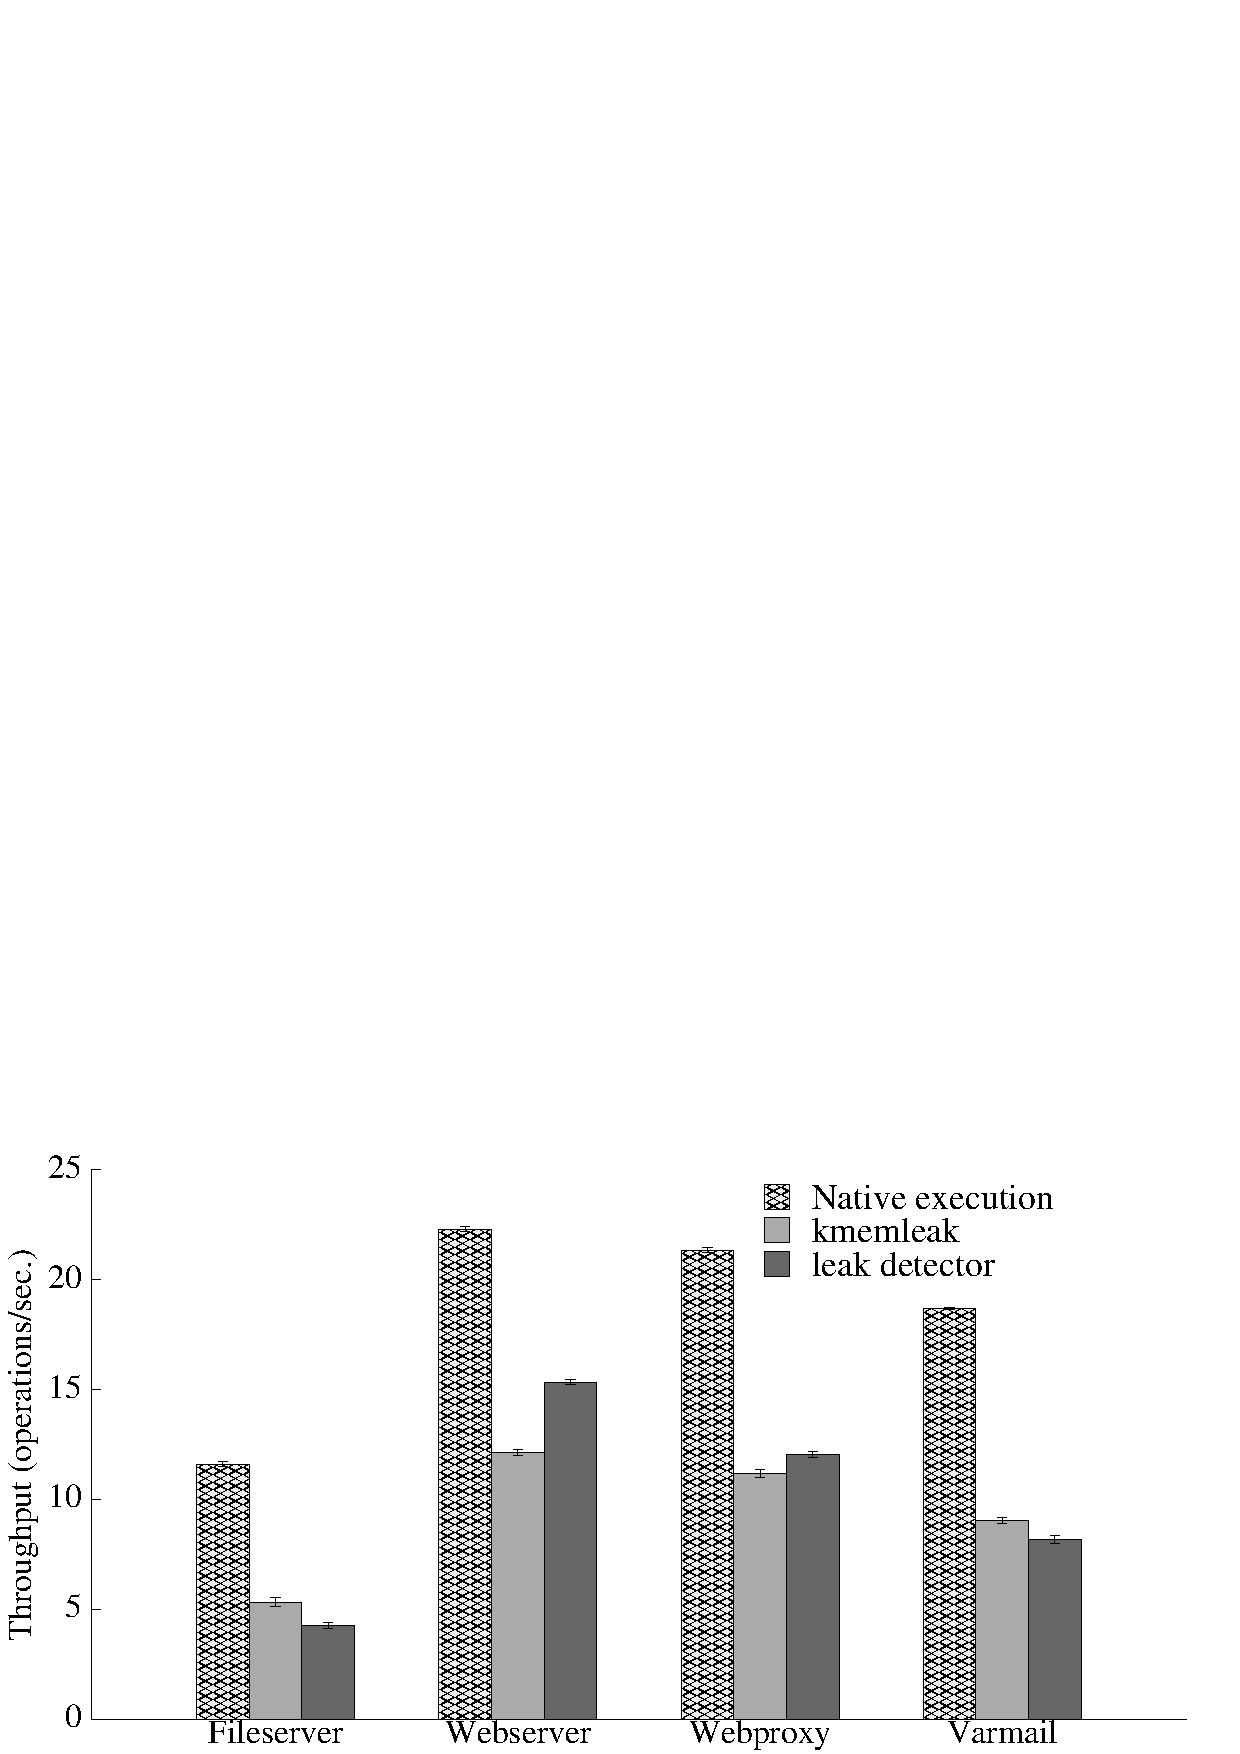
\includegraphics[width=6.0in,height=3.0in]{kmemleak.pdf}
\end{center}
\caption[Performance impact of leak detector on Filebench server benchmarks.]{\label{fig:leak_detector-kmemleak}The performance overhead of our leak detector when using the Filebench benchmark. It also compares the overhead of leak detector with \emph{kmemleak}, which operates on the entire kernel.}
\end{figure}
